\documentclass[mathserif]{beamer}
\usepackage{beamerthemeshadow}
\usepackage{beamerthemesplit}
%\usetheme{shadow}
\usecolortheme{default}
\setbeamertemplate{footline}[frame number]
\useinnertheme[shadow=true]{rounded}
%\setbeamertemplate{footline}{\insertframenumber/\inserttotalframenumber}
%\useoutertheme{infolines}
%\setbeamertemplate{headline}{} % removes the headline that infolines inserts

%\usetheme{boxes}
%\usepackage{amsmass}
%\usepackage{amssymb,amsfonts,url}

\usepackage{algorithm}
\usepackage{algorithmic}

\usepackage{graphicx}
\graphicspath{{Problems/}}


\title{CS711008Z  Algorithm Design and Analysis }
\subtitle{ Lecture 4. {\bf NP} and intractability (Part II) 
%\footnote{The slides were prepared based on Introduction to algorithms, Algorithm design, Computer and Intractability, and slides by Kevin Wayne with permission.} 
}
\author{Dongbo Bu \\
\ \ \ \ \ \ \ \ \ \ \ \ \ \ \ \ \ \ \ \ \ \ \ \ \ \ \ \ \ \ \ \ \ \ \ \ \ \ \ \ \ \ \ \ \ \ \ \ \ \ \ \ \ \ \ \ \ \ \ \ \ \ \ \ \ \ \ \ \ \ \ \ \ \ \ \ \ \ \ \ \ \ \ \ \ \ \ \ \ \ \ \ \ \ \ \ \ \ \ \  \\
{\small Institute of Computing Technology \\ Chinese Academy of Sciences, Beijing, China}}
\date{}

\begin{document}
%\begin{CJK}{UTF8}{cyberbit}

\frame{\titlepage}

\frame{
\frametitle{Outline}
\begin{itemize}
 \item Reduction: understanding the relationship between different problems. $A
\le_P B$ implies  ``B is harder than A''. 
 \item Problem classes: {\bf P}, {\bf NP}, {\bf coNP}, {\bf L}, {\bf NL}, {\bf PSPACE}, {\bf EXP}, etc. 
 \item {\sc Circuit Satisfiability} is one of the hardest problems in {\bf NP} class. 
 \item {\bf NP-Complete} problems
\end{itemize}
}

\frame{
\frametitle{ Complexity classes  }
\begin{itemize}
\item A complexity class of problems is specified by several parameters: 
\begin{enumerate}
 \item Computation model: multi-string Turing machine; 
 \item Computation mode: When do we think a machine accepts its input?
deterministic or non-deterministic?
 \item Computation resource: time, space. 
 \item Bound: a function $f$ to express how many resource can we use. 
 \end{enumerate}
\item The complexity class is then defined as the set of all languages decided by a multi-string Turing machine $M$ operating in the
deterministic/non-deterministic mode, and such that, for input $x$, $M$ uses at
most $f(|x|)$ units of time or space. 
\end{itemize}
(See ppt for description of Turing machine.)
}


\frame{ 
\frametitle{ Deterministic versus nondeterministic } 
\begin{itemize}
\item 
\textcolor{red}{\bf DTM}: In a deterministic Turing machine, the set of rules prescribes at most one action to be performed for any given situation. 
\item \textcolor{red}{\bf NTM}: A non-deterministic Turing machine (NTM), by contrast, may have a set of rules that prescribes more than one actions for a given situation. 
\item For example, a non-deterministic Turing machine may have both "If you are in state 2 and you see an 'A', change it to a 'B' and move left" and "If you are in state 2 and you see an 'A', change it to a 'C' and move right" in its rule set.
\end{itemize}
} 

\frame{
\frametitle{ Example: NFA and DFA } 
\begin{figure}
 \begin{minipage}{0.4\textwidth}
 \includegraphics[width=\textwidth] {NFA.eps} 
 \end{minipage}
 \begin{minipage}{0.4\textwidth}
 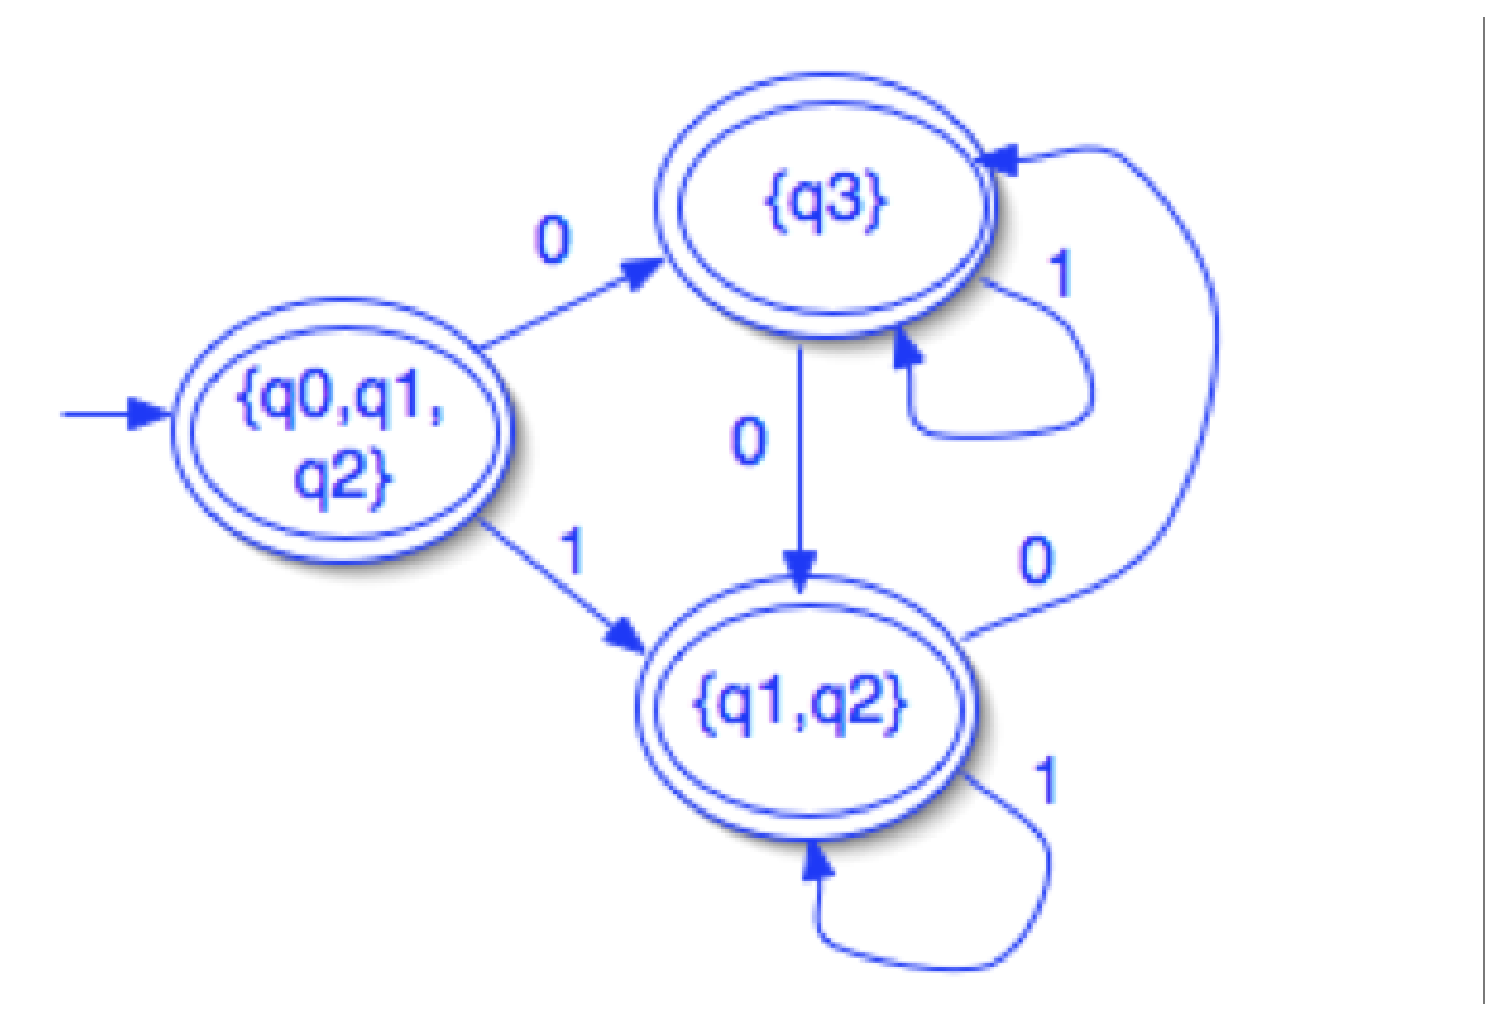
\includegraphics[width=\textwidth] {DFA.eps} 
\end{minipage}
\caption{NFA and DFA} 
\end{figure}
\begin{itemize}
\item 
Perhaps the easiest way to understand determinism and nondeterminism is by looking at NFA and DFA. 
\item 
In a DFA, every state has exactly one outgoing arrow for every letter in the alphabet.
\item 
However, the NFA in state 1  has two possible transitions for the letter "b".
\end{itemize}  
}

 
%
%\frame{ 
%\frametitle{ Complexity classes cont\'d}
%\begin{enumerate}
% \item {\bf TIME(f)}: deterministic Turing machine, time 
%\item {\bf NTIME(f)}: nondeterministic Turing machine, time. 
%\item {\bf SPACE(f)}: deterministic Turing machine, space. 
%\item {\bf NSPACE(f)}: nondeterministic Turing machine, space. 
%\end{enumerate}
%\begin{itemize}
% \item {\bf P}:  {\bf P = TIME($n^k$) = $\bigcup_{j>0}$ TIME($n^j$)} 
% \item {\bf{\bf NP}}:  {\bf{\bf NP} = NTIME($n^k$) = $\bigcup_{j>0}$ NTIME($n^j$)} 
% \item {\bf PSPACE}:  {\bf PSPACE = SPACE ($n^k$) } 
% \item {\bf NPSPACE}:  {\bf NPSPACE = NSPACE ($n^k$) }
% \item {\bf L}:  {\bf L = SPACE ($\log n $) } 
% \item {\bf NL}:  {\bf NL = NSPACE ($\log n $) } 
% \item {\bf EXP}:  {\bf EXP = TIME($2^{n^k}$) }
%\end{itemize}
%} 



\frame{
\frametitle{DTM vs. NTM: the difference between \textcolor{red}{finding} and \textcolor{red}{verifying} a solution}

\begin{figure}
 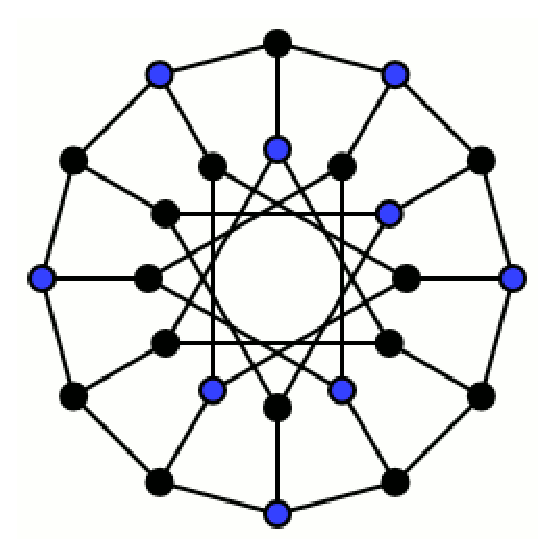
\includegraphics[width=1.5in] {Independent_set_graph.eps}
\end{figure}

\begin{itemize}
\item Consider the {\sc Independent Set} problem: does the given graph have an independent set of 9 nodes?
\item If your answer is ``\texttt{Yes}", you just need to provide a \textcolor{red}{\bf certificate} having 9 nodes. 
\item \textcolor{red}{\bf Certifier:} it is easy to verify whether the certificate is correct, i.e., the given 9 nodes form an independent set for this graph of 24 vertices. 
\item \textcolor{red}{\bf Solver:} However, it is not easy to find this independent set. 
\end{itemize}
}

\frame{
\frametitle{Another example}



% \begin{figure}
%  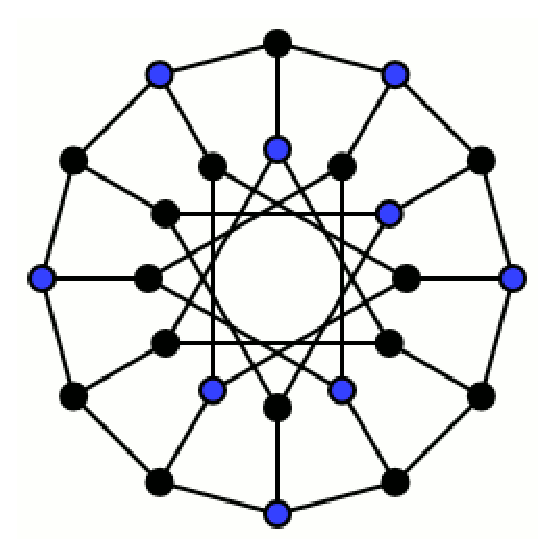
\includegraphics[width=1.5in] {Independent_set_graph.eps}
% \end{figure}

\begin{itemize}
\item Consider the following problem: does the formula $f(x)=x^5 - 3x^4 + 5x^3 -7x^2 + 11x -13 = 0$ have a real-number solution?
\item If your answer is ``\texttt{Yes}'', you just need to provide a \textcolor{red}{\bf certificate}, say $x=0.834...$.
\item  \textcolor{red}{\bf Certifier:} it is easy to verify whether the certificate is correct, i.e., $f(x)=0$. 
\item  \textcolor{red}{\bf Solver:} however, it is not easy to get a solution. 
\end{itemize}
}

\frame{
\frametitle{ {\bf P}  class }
\begin{itemize}
 \item 
{\bf P}: decision problems for which there is a polynomial-time algorithm to  \textcolor{red}{\bf solves}  it. 
\item 
Here, we say that an algorithm $A$ \textcolor{red}{\bf solves} problem $X$ if for all instance $s$ of $X$,  $A(s)=$ \texttt{YES} iff $s$ is a \texttt{YES}instance. 
\item 
Time-complexity: $A$ runs in polynomial-time if for \textcolor{red}{\bf every} instance $s$, $A(s)$ ends in at most $polynomial(|s|)$ steps. 
 \item {\sc Stable Matching} problem:  $O(n^2)$. 
\end{itemize}
}

\frame{
\frametitle{ {\bf NP}  class }
\begin{itemize}
 \item 
{\bf NP}: decision problems for which there exists a polynomial-time \textcolor{red}{\bf certifier}. \footnote{{\bf NP}  denotes ``non-deterministic polynomial-time''. This is just simple but equivalent definition.}
\item 
Here we say that an algorithm $C(s, t)$ \textcolor{red}{\bf certificates} problem $X$ if for each ``\texttt{YES}'' instance $s$, there exists a \textcolor{red}{\bf certificate} $t$ such that $C(s, t) = $\texttt{YES}, and $|t| = polynomial(|s|)$. 
\item
\textcolor{red}{\bf Certificate}: an evidence to demonstrate this instance is \texttt{YES};
\end{itemize}

\begin{itemize}

\item Note: a certifier approach the problem from a \textcolor{red}{\bf managerial} point of view as follows:
\begin{itemize}
 \item It will not actually try to solve the problem directly; 
 \item Rather, it is willing to efficiently evaluate proposed ``proof''. 
\end{itemize}
\end{itemize}

}

\frame{
\frametitle{Certificate and certifier for {\sc Hamilton Cycle} problem}

\begin{itemize}
 \item 
Problem: Is there a Hamiltonian cycle in the give graph? 
\item 
If your answer is \texttt{YES}, you just need to provide a certificate, i.e. a permutation of $n$ nodes; 
\item 
Certifier: checking whether this path forms a cycle;
\item Example: 




 \item Certifier: it takes polynomial time to verify the certificate.  Thus {\sc Hamilton Cycle} is in {\bf NP}  class. 
 \end{itemize}
\begin{figure}
 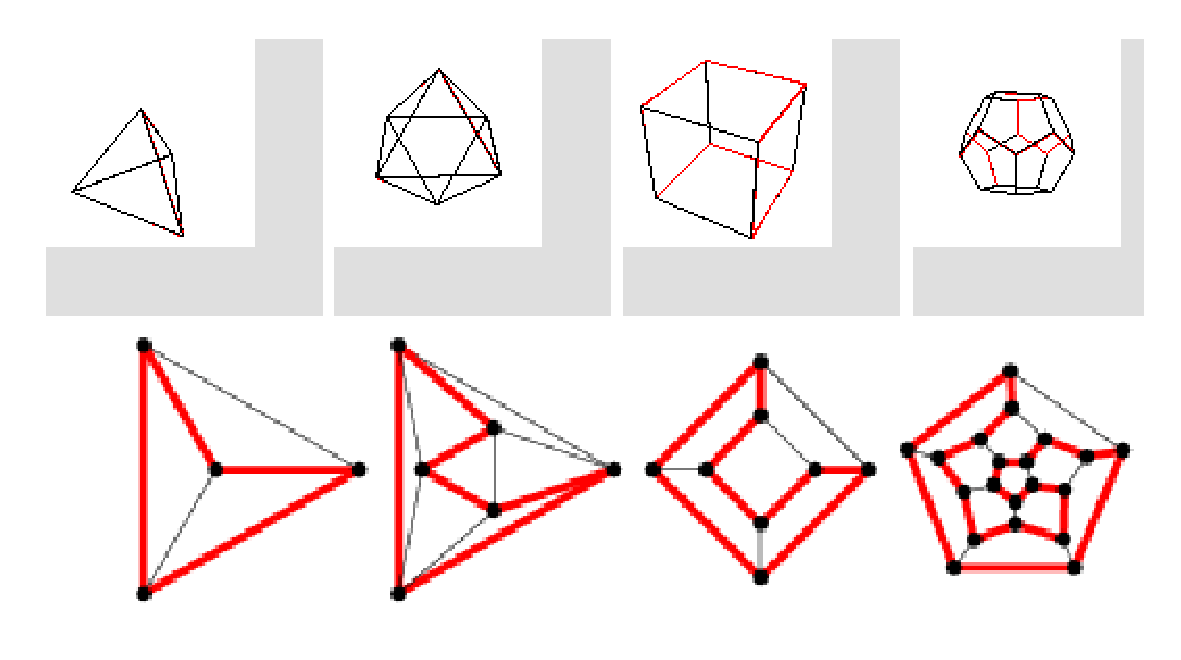
\includegraphics[width=2.5in]{L3-hamiltoncycle2.eps}
\end{figure}
}

\frame{
\frametitle{Certificate and certifier for {\sc SAT} problem }
\begin{itemize}
\item 
Problem: Is the given {\bf CNF} satisfiable?
\item 
If your answer is \texttt{YES}, you just need to provide a certificate, i.e.  an assignment for all $n$ boolean variables;
\item
Certifier: checking whether each clause is satisfied by this assignment;

\item 
Example: 

\begin{itemize}
\item 
 An instance: $( x_1 \vee \neg x_2 \vee x_3 ) \wedge ( \neg x_1 \vee x_2 \vee x_3 ) $
\item
 Certificate: $x_1 = \texttt{TRUE}, x_2 = \texttt{TRUE}, x_3 = \texttt{FALSE}$;
 \item Certifier: it takes polynomial time to verify the certificate.  Thus {\sc SAT} is in {\bf NP}  class. 
 \end{itemize}
\end{itemize}

}

\frame{
\frametitle{The ``certificate'' idea is not entirely trivial. }
\begin{enumerate}
 \item 

For {\sc UNSAT} problem, it is difficult to provide a short ``certificate'':
\begin{itemize}
 \item 
Suppose we want to prove a {\sc SAT} instance is \textcolor{red}{\bf unsatisfiable}, what evidence could convince you, in polynomial time,  that the instance is unsatisfiable? 
\end{itemize}

\item In addition, we can also transform a \textcolor{red}{{\bf certifier}} into an  \textcolor{red}{{\bf algorithm}}. 
\begin{itemize}
 \item 
A certifier can be used as the core of a ``brute-force'' algorithm to solve the problem: enumerate all possible certificate $t$ in $O(2^{|t|})$ time, and run $C(s, t)$. It will take exponential-time.  \\
\end{itemize}
\end{enumerate}
}

\frame{
\frametitle{ Problem classes: {\bf P}, {\bf NP}, and {\bf EXP}}
Three classes of problems: 
\begin{itemize}
\item 
{\bf P:}  decision problems for which there is a polynomial-time \textcolor{red}{algorithm}; \\
\item 
{\bf NP:} decision problems for which there is a polynomial-time \textcolor{red}{certifier}; \\
\item 
{\bf EXP:}  decision problems for which there is an \textcolor{red}{exponential-time} algorithm; \\
\end{itemize}
} 

\frame{
\frametitle{  ${\bf P}  \subseteq {\bf NP}$ } 
\begin{theorem}
 ${\bf P}  \subseteq {\bf NP}$.
\end{theorem}
\begin{Proof}
\begin{itemize}
 \item 
 Consider any problem $X$ in {\bf P}; \\
 \item 
There is an algorithm $A$ to solve it;  \\
 \item 
 We design a certifier $C$ as follows:  when presented with input $(s, t)$, simply return $A(s)$. 
\end{itemize}
\end{Proof}
}
\frame{
\frametitle{ $ {\bf NP} \subseteq {\bf EXP}$ } 
 
\begin{theorem}
 $ {\bf NP} \subseteq {\bf EXP}$.
\end{theorem}
\begin{Proof}
\begin{itemize}
 \item 
 Consider any problem $X$ in {\bf NP} ; \\
 \item 
There is a polynomial-time certifier $C$ to certificate it;  \\
\item 
 For an instance $s$, run $C(s, t)$ on \textcolor{red}{\bf all} possible certificates $t$, $|t| = polynomial(|s|)$; \\ 
\item 
Return \texttt{Yes} if $C(s, t)$ returns \texttt{Yes} for any certificate $t$. 
\end{itemize}
\end{Proof}
}


\frame{
\frametitle{} 
\begin{block}{ Question 1: {\bf P = NP?} }
%If {\bf P = NP}, then for a ``Yes" instance, an efficient ``verifying'' a certificate means an efficient ``finding'' a solution. 
\end{block}
}


\frame{
\frametitle{ {\bf P} vs. {\bf NP}  }
\begin{itemize}
 \item 
The main question: ${\bf P}  ={\bf NP}?$  [S. Cook]
\item 
In other words, is \textcolor{red}{solving} a problem as easy as \textcolor{red}{certificating} an evidence? 
\begin{itemize}
 \item 
If {\bf P = NP}, then for a ``Yes" instance, an efficient ``verifying'' a certificate means an efficient ``finding'' a solution, and there will be  efficient algorithms for {\sc SAT, TSP, Hamilton Cycle}, etc.
\item 
If {\bf P $\neq$ NP}: there is  no efficient algorithms for these problems; 
\end{itemize}


\item 
Clay \$7 million prize. (See http://www.claymath.org/millennium/P\_vs\_NP/ )
\end{itemize}

\begin{figure}
 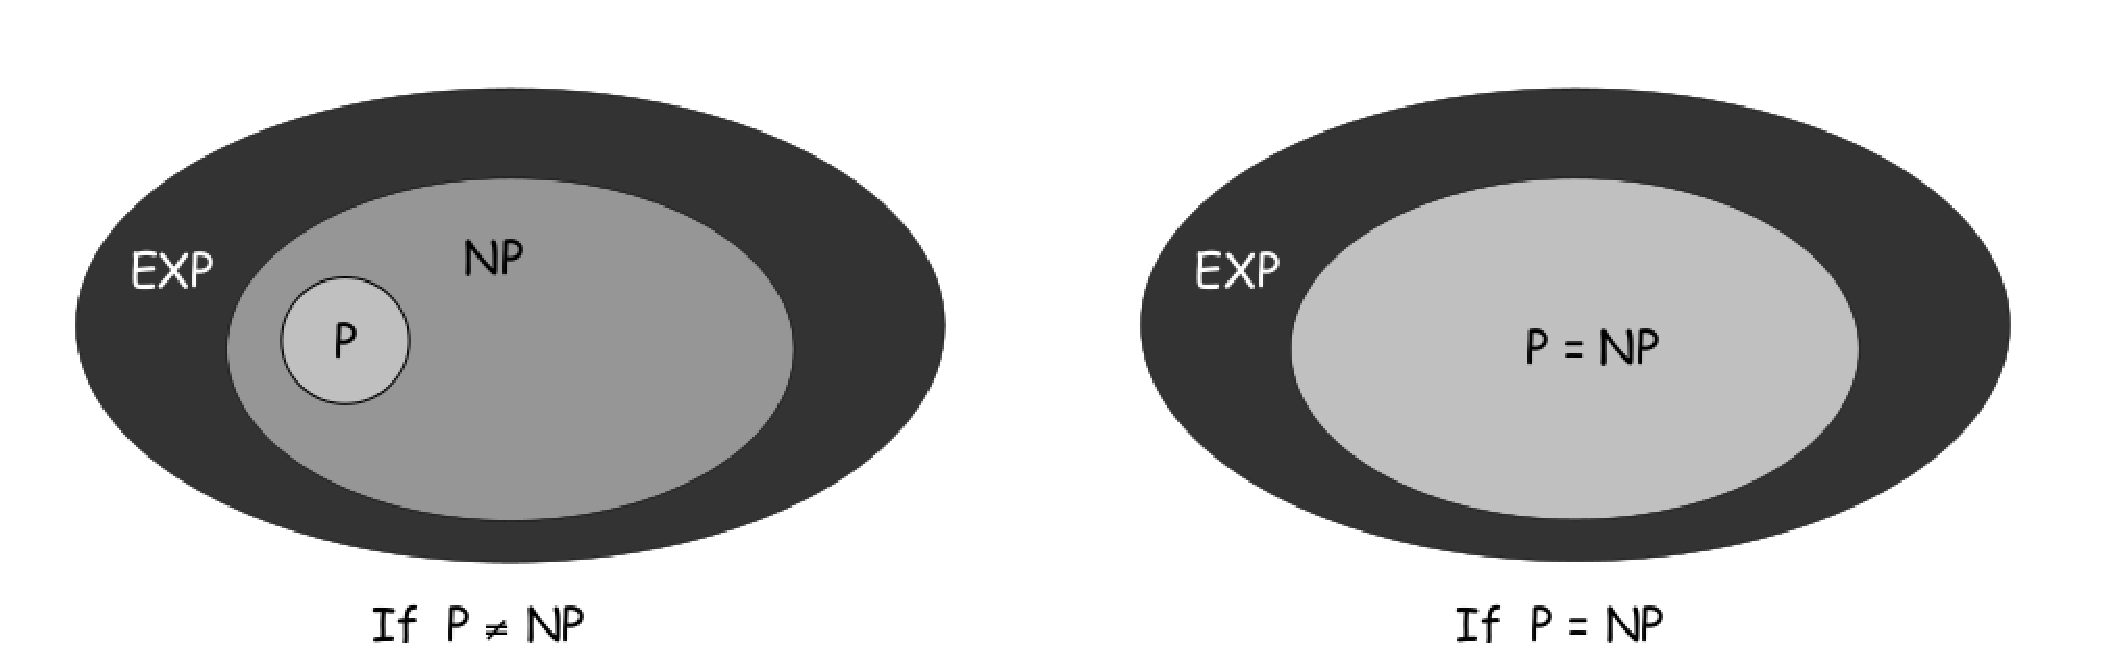
\includegraphics[width=3in]{L3-PNP.eps}
\end{figure}


}


\frame{
\frametitle{}
\begin{block}{}
 A first NP-Complete problem
\end{block}
}

\frame{
\frametitle{${\bf NP-complete}$ class: the hardest problem in {\bf NP}  class}
\begin{itemize}
 \item Due to the absence of progress of {\bf P=NP?} question, a more approachable
question was posed: \\
	What is the hardest problems in {\bf NP}? 
\item This is approachable since by using polynomial-time reduction, one can find connection between problems, and
gain insight of the structure of {\bf NP}  class. 
\item The hardest problems in the $NP$ class:
\begin{itemize}
\item 
{\bf NP-hard}: a problem $Y$ is {\bf NP-hard}  if for \textcolor{red}{\bf any}
{\bf NP} problem $X$, $X \le_p Y$;
\item 
{\bf NP-complete}: a problem $Y$ is in {\bf NP}, and is {\bf NP-hard}. 
\end{itemize}
\end{itemize}
}

\frame{
\frametitle{    }
\begin{theorem}
 Suppose $Y$ is a {\bf NP-complete} problem. $Y$ is solvable in polynomial-time
  iff {\bf P=NP}
\end{theorem}
\begin{Proof}
\begin{itemize}
 \item 
Let $X$ be any problem in {\bf NP} ; 
 \item 
Since $X \le_P Y$, $X$ can be solved in polynomial-time through the ``reduction
algorithm''. 
%\item Conversely, Obvious. Since $Y$ is also in {\bf NP}. 
\end{itemize}

\end{Proof}
\begin{itemize}
 \item 
Consequence: if there is any problem in {\bf NP}  that cannot be solved in
polynomial-time, then no NP-Complete can be solved in polynomial-time. 
\end{itemize} 
}

\frame{
\frametitle{ The first NP-Complete problem [Cook, Levin 1971] }
\begin{itemize}
 \item 
It is not at all obvious that {\bf NP-complete} problems should even exist. 
\item 
Two possible cases: 
\begin{enumerate}
 \item two incomparable problem $X'$ and $X''$, and there is $no$ problem $X$
such that $X' \le_P X$, and $X'' \le_P X$? 
 \item an infinite sequence of problems $X_1 \le_P X_2 \le_P ... $; 
\end{enumerate}

\item The difficulty is to prove that \textcolor{red}{\bf any } {\bf NP} problem $X$
can be reduced to a {\bf NP-complete} problem. 
\end{itemize}
}

\frame{
\frametitle{S. Cook and L. Levin} 

\begin{figure}
 \begin{minipage}{0.3\textwidth}
 \includegraphics[width=\textwidth] {Cook.eps} 
 \end{minipage}
 \begin{minipage}{0.3\textwidth}
 \includegraphics[width=\textwidth] {Levin.eps} 
\end{minipage}
\caption{Stephen Cook and Leonid Levin} 
\end{figure}

In 1982, Cook received the Turing award. His citation reads:
\begin{small}
{\it For his advancement of our understanding of the complexity of computation in a significant and profound way. His seminal paper, The Complexity of Theorem Proving Procedures,..., laid the foundations for the theory of NP-Completeness. The ensuing exploration of the boundaries and nature of NP-complete class of problems has been one of the most active and important research activities in computer science for the last decade.}
\end{small}
} 

\frame{
\frametitle{Let's show {\sc Circuit Satisfiability} is {\bf NP-complete} }
\begin{itemize}
\item {\sc Circuit:} a labeled, directed acyclic graph to simulate computation process on
physical circuit. 
\end{itemize} 

\begin{block}{{\sc Circuit Satisfiability} problem }
 {\bf INPUT:}  a circuit; \\
 {\bf OUTPUT:}  is there an assignment of input making output to be 1?
\end{block}

\begin{figure}
 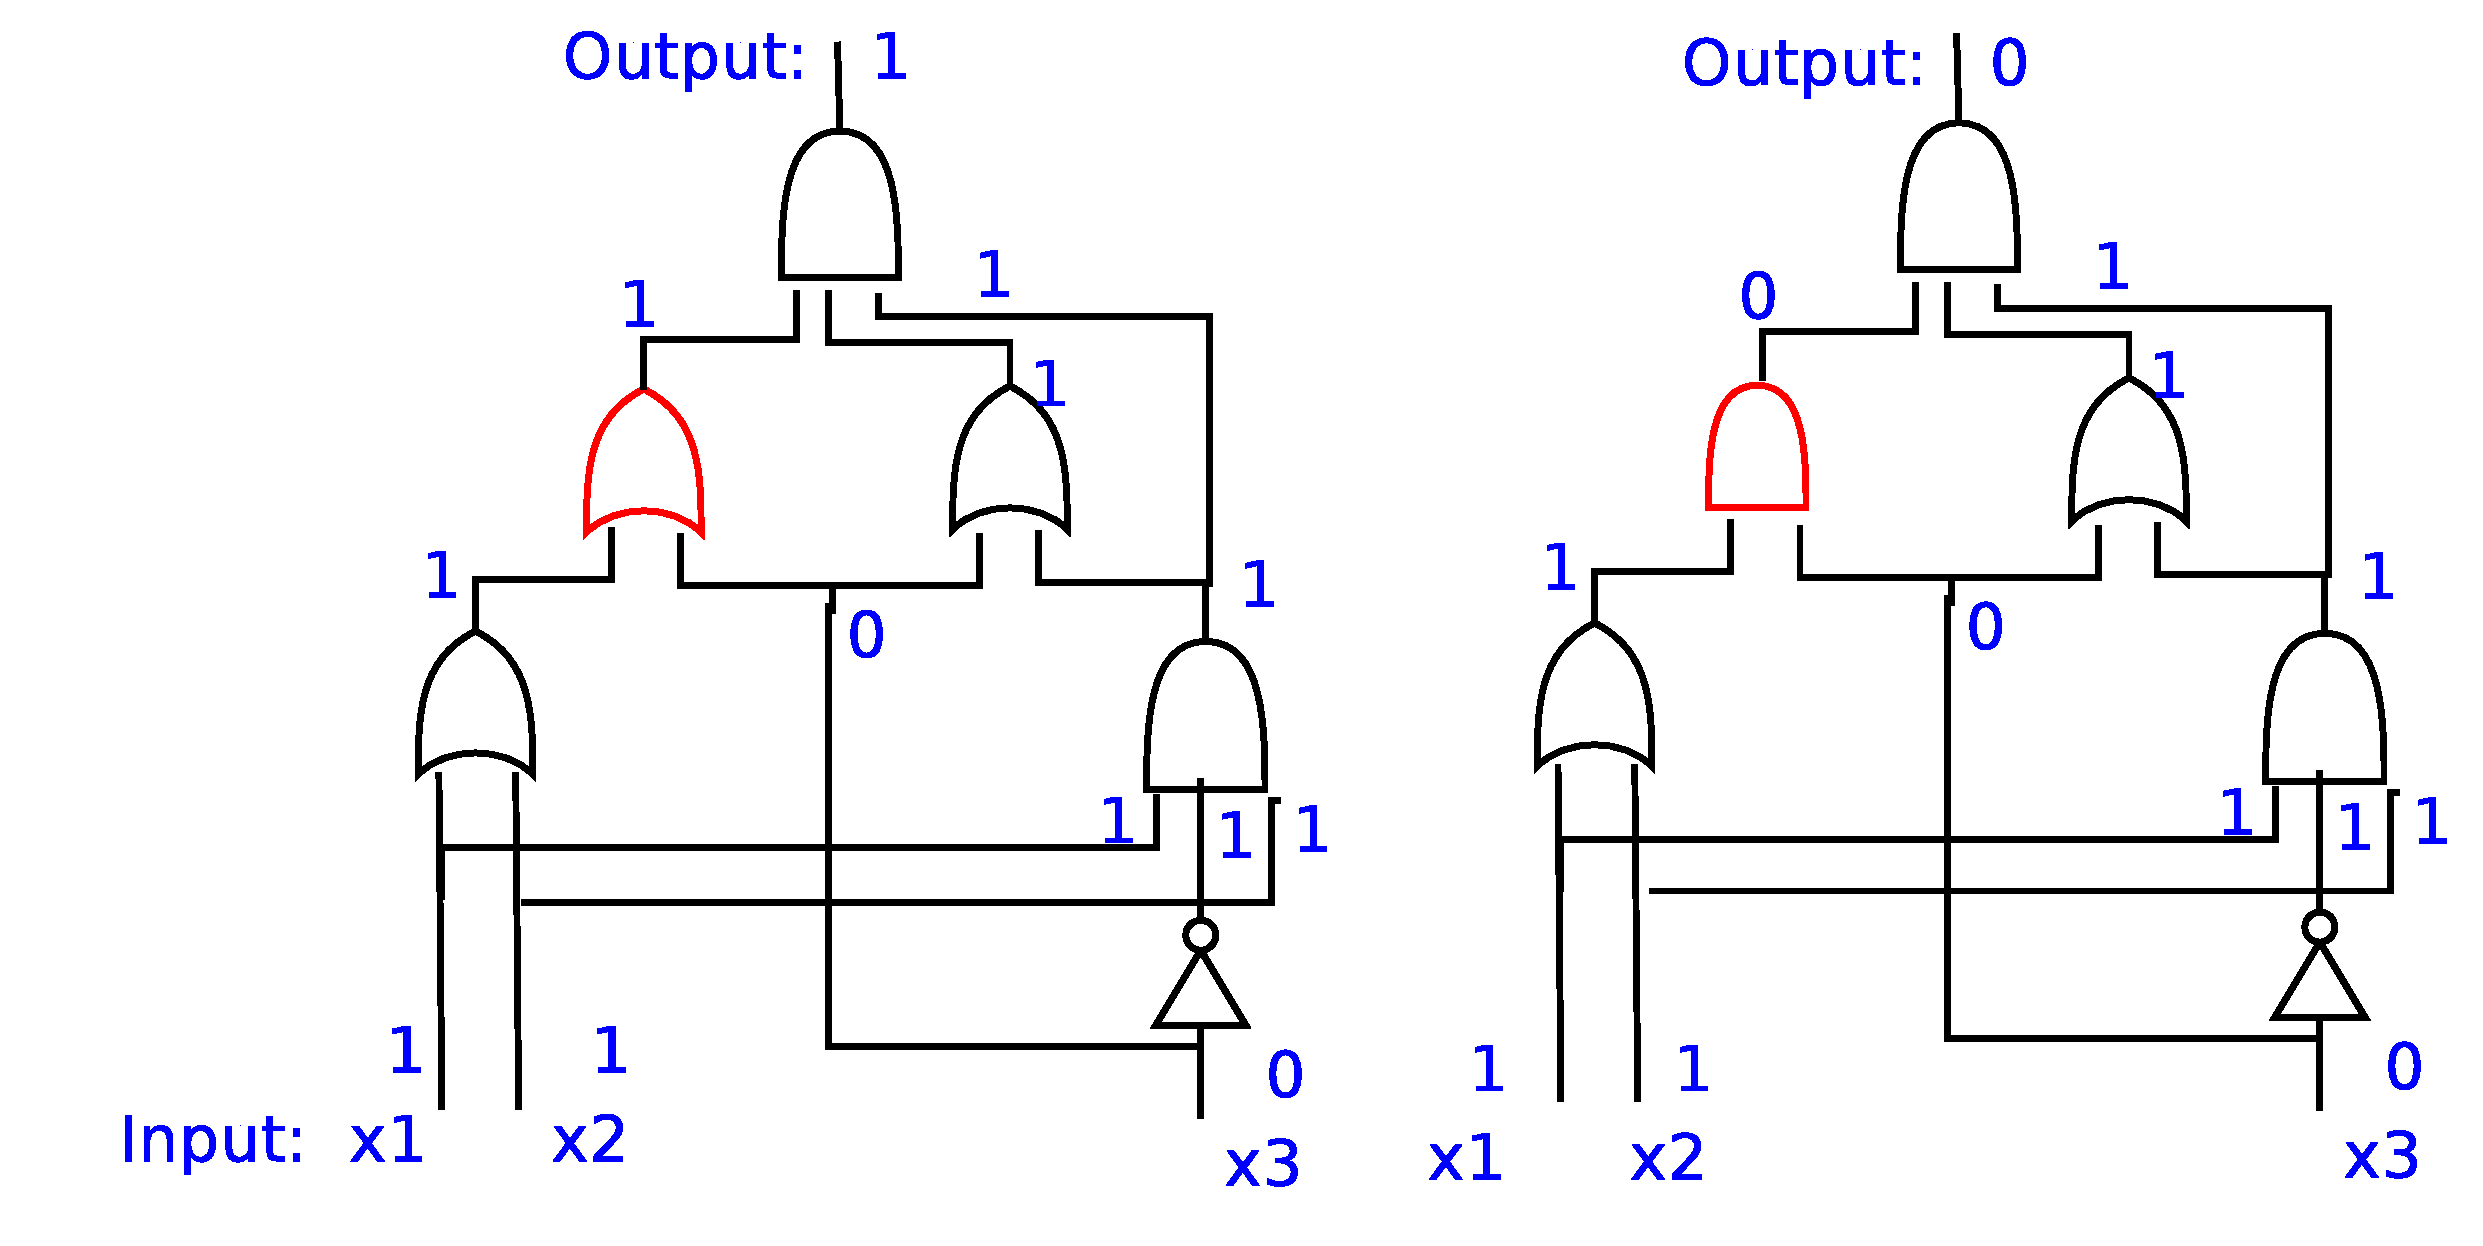
\includegraphics[width=2.3in]{L4-circuit-example-sat.eps}
 \caption{Left: satisfiable. Right: unsatisfiable. }
\end{figure}

}

\frame{
\frametitle{{\sc Circuit Satisfiability}  cont'd}
\begin{block}{{\sc Circuit Satisfiability} problem }
 {\bf INPUT:}  a circuit; \\
 {\bf OUTPUT:}  is there assignment of input that cause the output to take the
value 1?
\end{block}

\begin{figure}
 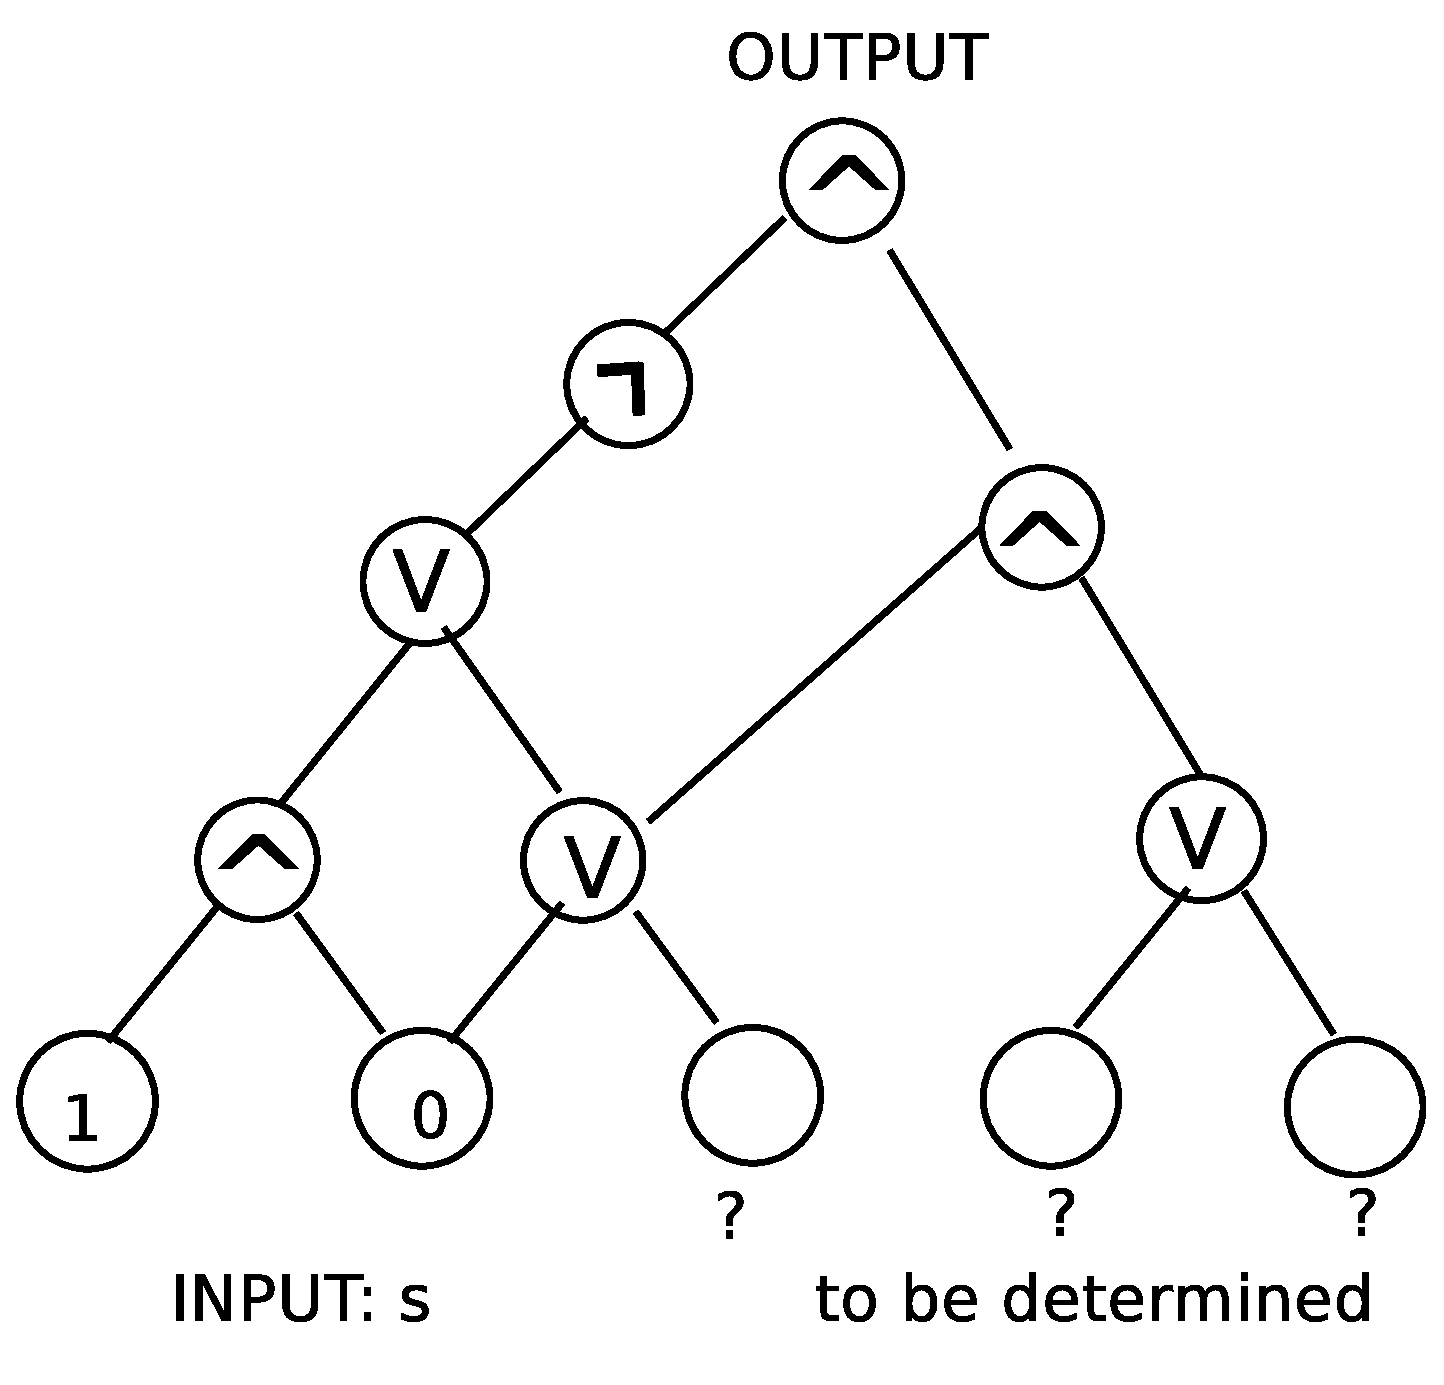
\includegraphics[width=1.5in]{L4-circuitexample.eps}
\end{figure}
%Is this circuit satisfiable? 
}


\frame{
\begin{block}{ {\sc Circuit Satisfiability} is the most natural problem. }

\begin{itemize}
 \item For example, {\sc Independent Set} problem can be reducible to {\sc
Circuit Satisfiability}.
 \item In other words, a circuit can be designed to simulate certifier of {\sc
Independent Set} problem, i.e., the circuit can be satisfied iff the {\sc
Independent Set} instance is a ``Yes'' instance.
\end{itemize}
\end{block}
}

\frame{
\frametitle{ {\sc Circuit Satisfiability} problem } 
{\sc Circuit Satisfiability} problem can be used to represent a large family of
problems, say  
 {\sc Independent Set} $\le_P$ {\sc Circuit Satisfiability}. 
\begin{figure}
 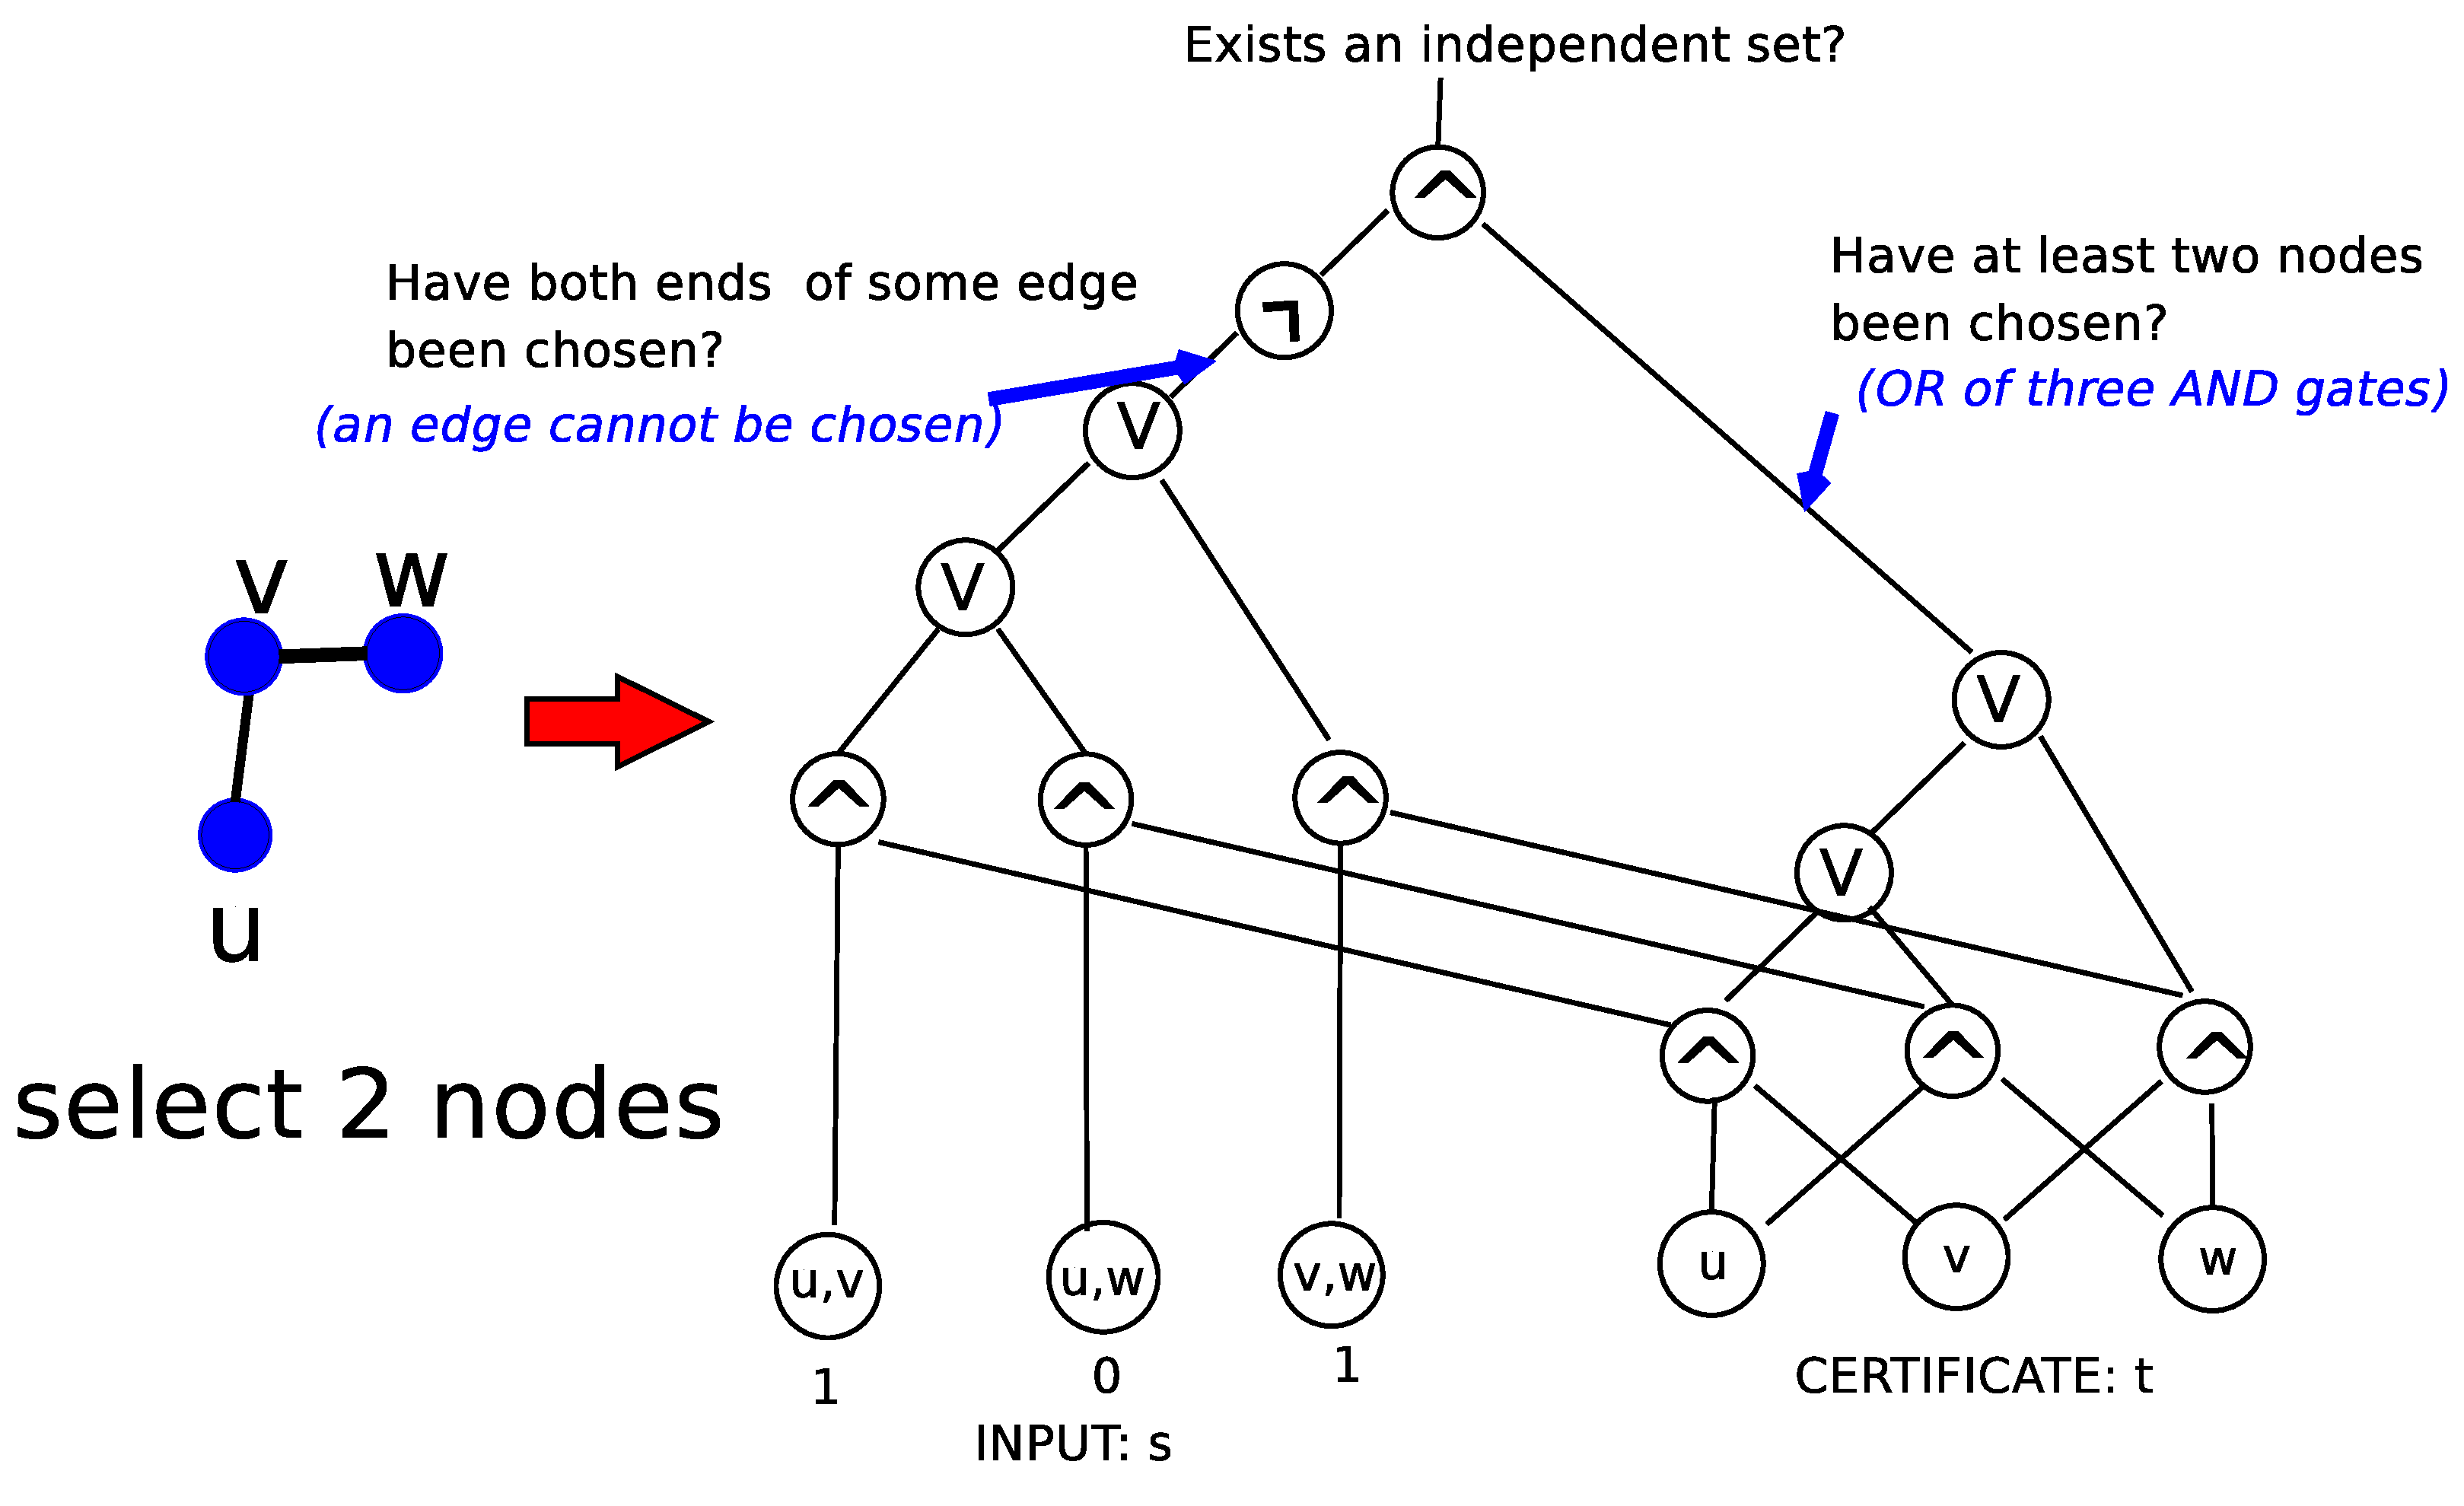
\includegraphics[width=3in]{L4-independentsetcircuit.eps} 
\end{figure}
\begin{itemize}
 \item Existing an independent set $\Rightarrow$ $C$ is satisfiable. 
 \item No independent set $\Rightarrow$ $C$ is unsatisfiable. 
\end{itemize}
}

\frame{
\begin{block}{ {\sc Circuit Satisfiability} is the most natural problem. }
\begin{itemize}
 \item In fact, besides {\sc Independent Set} problem, \textcolor{red}{ALL} {\bf
NP} problems can be reducible to {\sc Circuit Satisfiability}. 
 \item In other words, specific circuits can be designed to simulate the
certifiers of \textcolor{red}{ALL} {\bf NP} problems.
 \item  {\sc Circuit Satisfiability} is NP-Complete.
\end{itemize}
\end{block}
}

\frame{
\begin{footnotesize}
\begin{scriptsize}
\begin{Theorem}
 {\sc Circuit Satisfiability} is NP-Complete.
\end{Theorem}
\begin{Proof}
\begin{itemize}
 \item We will show for any problem $X\in NP$, $X \le_P $ {\sc Circuit-Sat}.
 \item Remember that $X \in NP$ implies a certifier $C(s,t)$ running in
$T(|s|)=poly(|s|)$ time. 
 \item And $s$ is a ``Yes'' instance of $X$ $\Leftrightarrow$ there is a
certificate $t$ of length $p(|s|)$ such that $C(s,t) = Yes$. 
 \item Our objective is to design a circuit that generates same output to the
certifier $C(s,t)$. 
 \item \textcolor{red}{Key idea: Represent the computation process of certifier
$C(s,t)$ as a sequence of configurations.} \begin{scriptsize}
 Here, configuration refers to any particular state of computer, including
program $C(s,t)$, program counter PC, memory, etc. ( You can image configuration
as the tape of a universal Turing machine.) \end{scriptsize}
 \item The $i$-th configuration is transformed to the $(i+1)$-st configuration
by a combinatorial circuit $M$ simulating CPU (in a single clock cycle). 
 \item \textcolor{red}{Simply paste $T(n)$ copies of $M$ to generate a single
circuit $K$.}
 \item When inputed with initial configuration, $K$ will generate
\textcolor{red}{ALL} configurations. 
 \item The output (a specific bit in working memory) appears on a pin. 
 \end{itemize}
\end{Proof}
\end{scriptsize}
\end{footnotesize}
}

\frame{
\frametitle{Certifier $\Rightarrow$ circuit: an example}
\begin{figure}
 \includegraphics[width=3.8in]{L4-programcircuit.eps}
\end{figure}
\begin{footnotesize}
\begin{itemize}
 \item Configuration: any particular state of computer, including program
$C(s,t)$, program counter PC, working memory, etc. 
 \item Transformation: simply connecting $T(n)$ copies of physical circuit $M$
to generate a single circuit. \\
\item 
 Note that both $\#$configuration and $\#$working$\_$memory are polynomial. 
 \end{itemize}
\end{footnotesize}
}
\frame{
\frametitle{Certifier $\Rightarrow$ circuit: an example}
\begin{figure}
 \includegraphics[width=3.8in]{L4-programcircuit-step0.eps}
\end{figure}
\begin{footnotesize}
 \begin{itemize}
  \item Equivalence: When inputed with the initial configuration, ALL
configurations will appear step-by-step (as how CPU does in a single clock
cycle).  Finally a specific pin outputs Yes/No.
 \end{itemize}
\end{footnotesize}
}
\frame{
\frametitle{Certifier $\Rightarrow$ circuit: Step 1}
\begin{figure}
 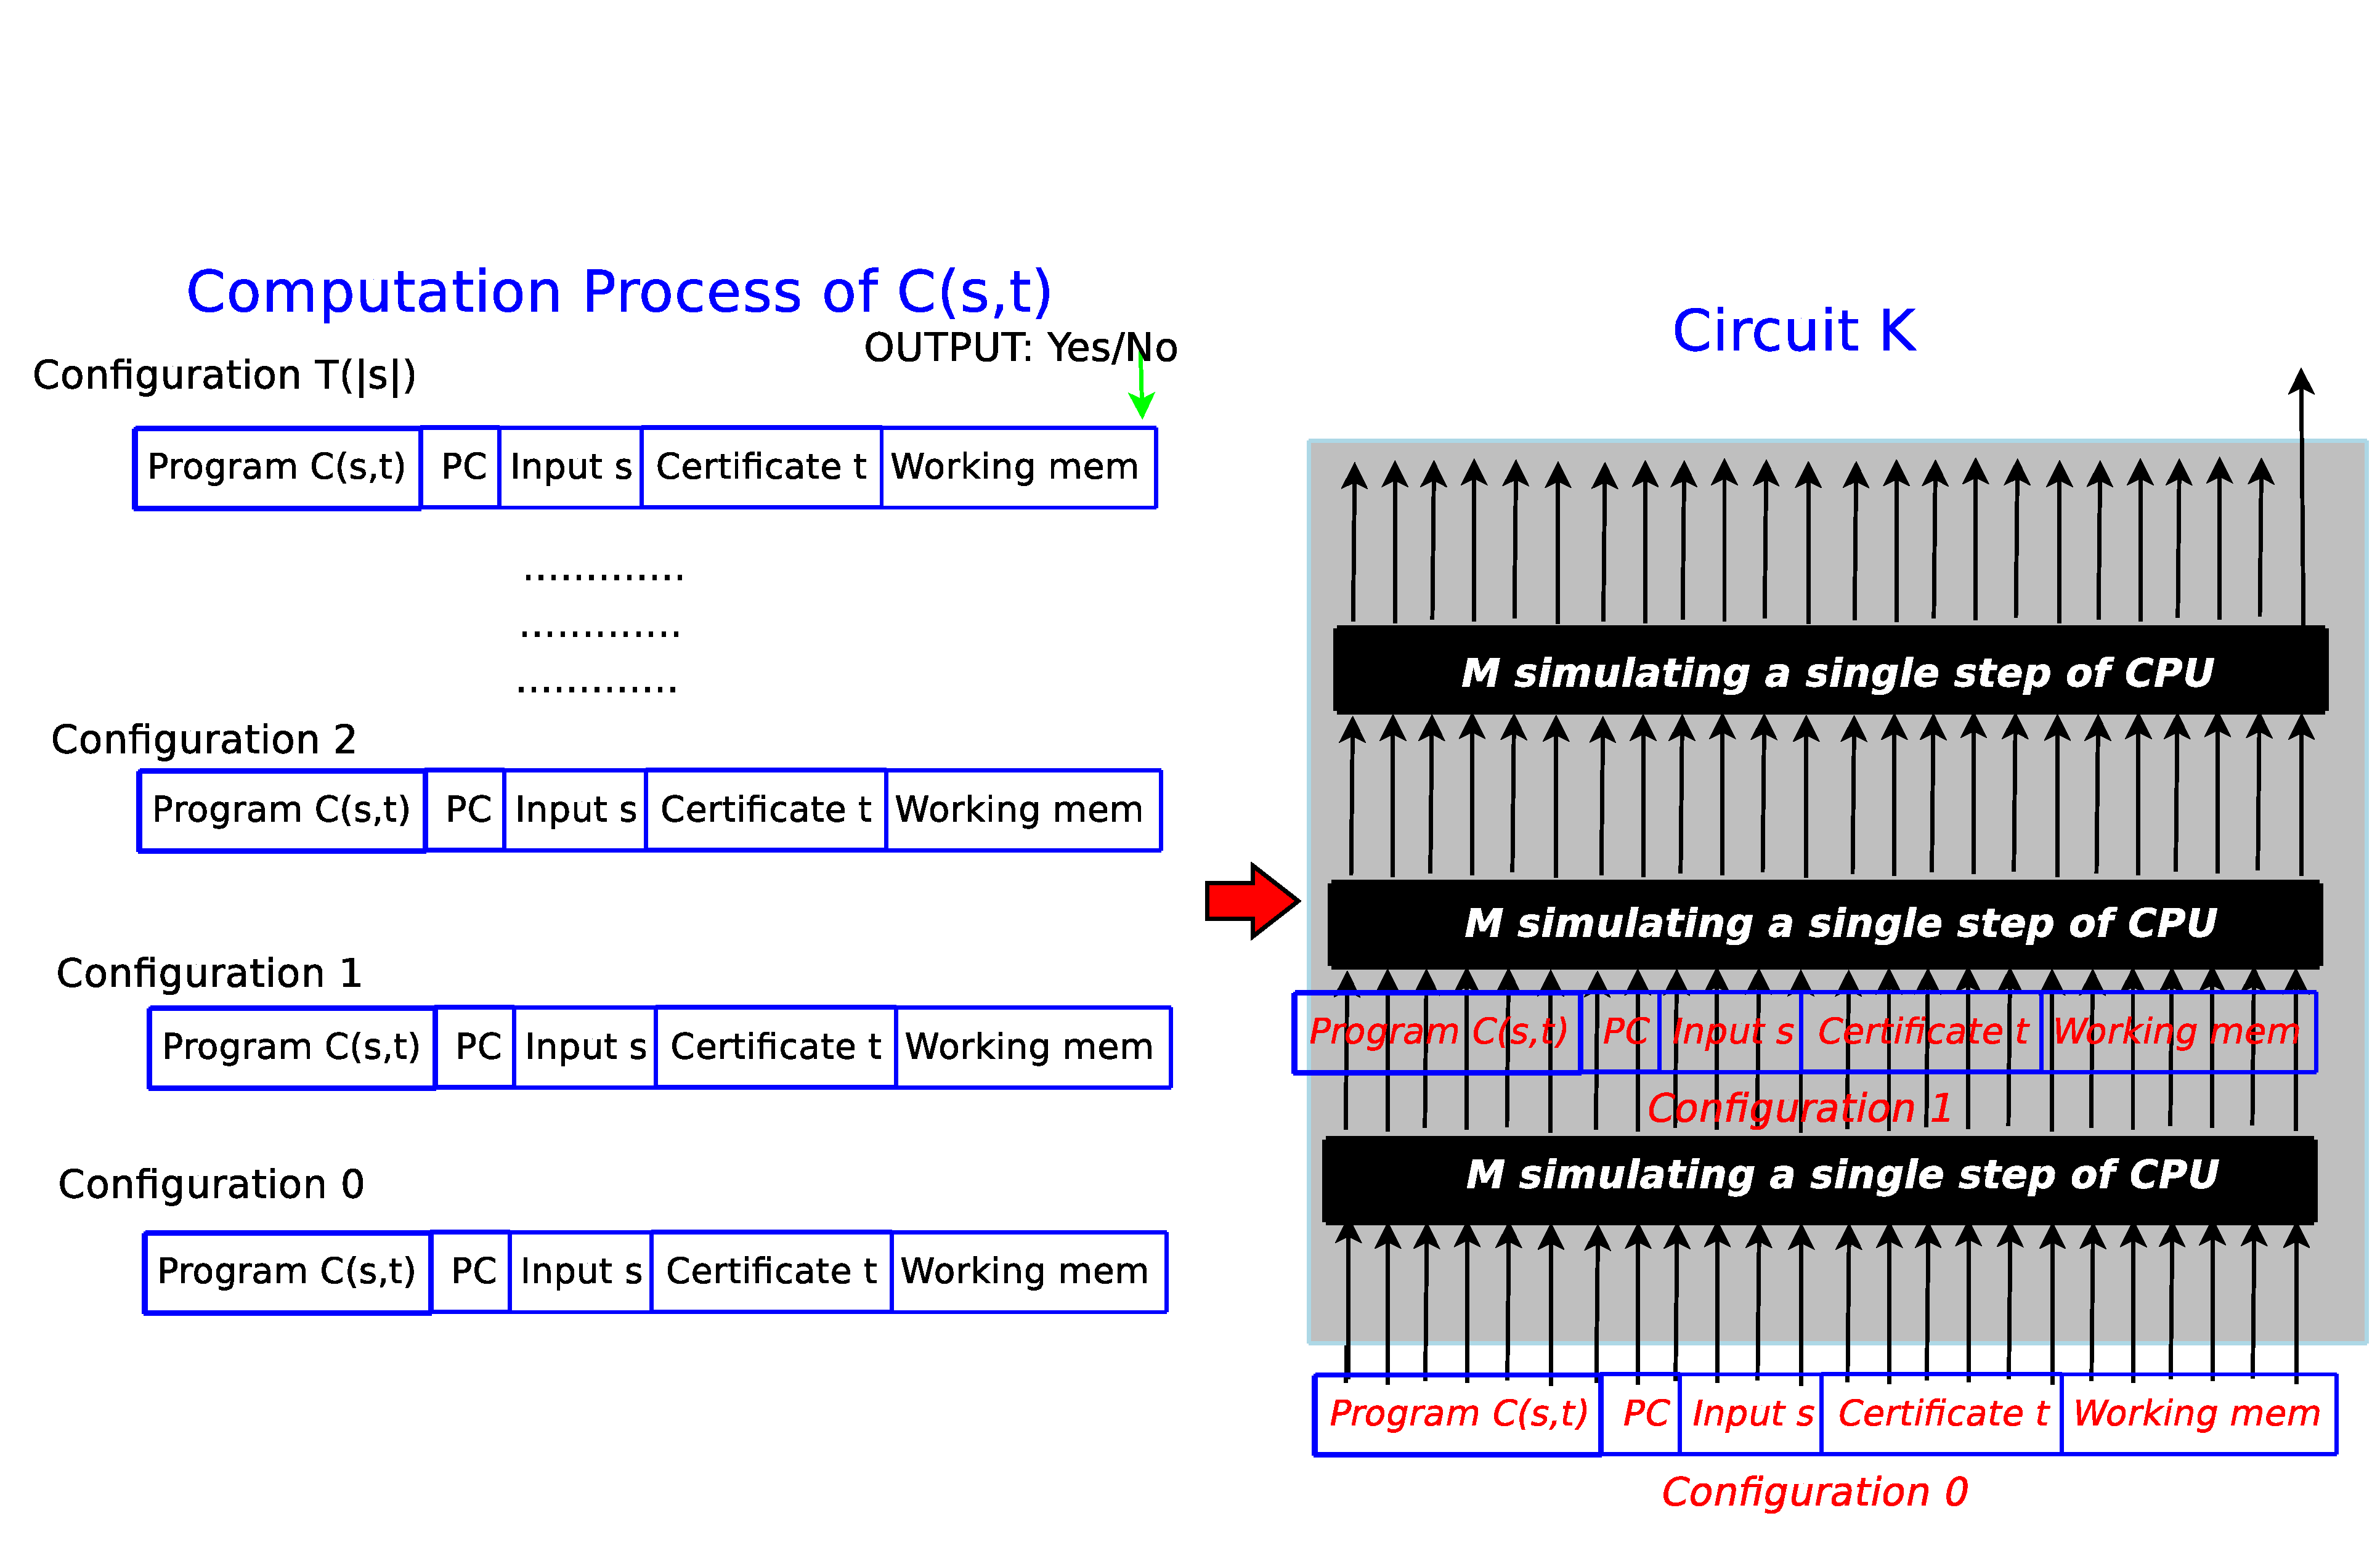
\includegraphics[width=4.0in]{L4-programcircuit-step1.eps}
\end{figure}
\begin{footnotesize}
 \begin{itemize}
 \item Equivalence: configuration 1 will appear in the second layers of pins
when inputed with initial configuration. 
 \end{itemize}
\end{footnotesize}
}

\frame{
\frametitle{Certifier $\Rightarrow$ circuit: Step 2}
\begin{figure}
 \includegraphics[width=4.0in]{L4-programcircuit-step2.eps}
\end{figure}
\begin{footnotesize}
 \begin{itemize}
 \item Equivalence: configuration 2 will appear in the third layers of pins when
inputed with initial configuration. 
 \end{itemize}
\end{footnotesize}
}

\frame{
\frametitle{Certifier $\Rightarrow$ circuit: Step $T(|s|)$}
\begin{figure}
 \includegraphics[width=4.0in]{L4-programcircuit-stepn.eps}
\end{figure}
\begin{footnotesize}
 \begin{itemize}
 \item Equivalence: configuration $T(|s|)$  will appear in the topest layers of
pins. A specific pin reports Yes/No. Thus, circuit $K$ outputs ``Yes''
$\Leftrightarrow$ certifier $C(s,t)$ reports ``Yes''.
 \end{itemize}
\end{footnotesize}
}

\frame{
\begin{block}{}
 Proving further NP-Complete problems
\end{block}
}

\frame{
\frametitle{Proving further  NP-Complete problems}

\begin{itemize}
\item 
Once we have a first {\bf NP-complete}, we can discover many more via the
following property:
\end{itemize}

\begin{theorem}
 If $Y$ is an {\bf NP-complete}, and $X$ is in {\bf NP} with the property
$Y\le_P X$, then $X$ is also NP-Complete.
\end{theorem}
\begin{itemize}
\item 
General strategy for proving new problem $X$ NP-Complete:
\begin{enumerate}
 \item Prove that $X$ is in NP;
 \item Choose an NP-Complete problem $Y$; 
 \item Consider an arbitrary instance $y$ of $Y$, and show how to construct, in
polynomial-time, an instance $x$ of $X$, such that $y$ is a ``Yes'' instance
$\Leftrightarrow$ $x$ is a ``Yes'' instance. 
\end{enumerate}
\end{itemize}

}


\frame{
\begin{Theorem}
 {\sc SAT} is {\bf NP-complete}.
\end{Theorem}
(Part 1: {\sc SAT} belongs to NP.)
\begin{Proof}
\begin{itemize}
 \item Certificate: assignment of variables. 
 \item Certifier: simply evaluate each clause and $\Phi$. 
\end{itemize}
\end{Proof}
e.g., $\Phi = ( x_1 \vee \neg x_2 \vee x_3)$ 
Certificate: $x_1 = T$ $x_2 = T$ $x_3 = T$.
}

\frame{
\begin{Theorem}
 {\sc SAT} is NP-Complete.
\end{Theorem}
(Part 2: {\sc SAT} is {\bf NP-hard}. In particular, {\sc Circuit
Satisfiability} $\le_P$ {\sc SAT})
\begin{Proof}
\begin{itemize}
 \item each wire in $C$ $\Rightarrow$ a variable; 
 \item a gate in $C$ $\Rightarrow$ a formula involving variables of incident
wires; 
 \item $\Phi$ is the $AND$ of output variable with the conjunction of clauses of
all gates.  
\item  The {\sc Circuit Satisfiability} instance is satisfied iff the
constructed {\sc SAT} instance is satisfied. 
\end{itemize}
\end{Proof}
} 
\frame{
\frametitle{{\sc Circuit Satisfiability} $\le_P$ {\sc SAT}}
\begin{figure}
 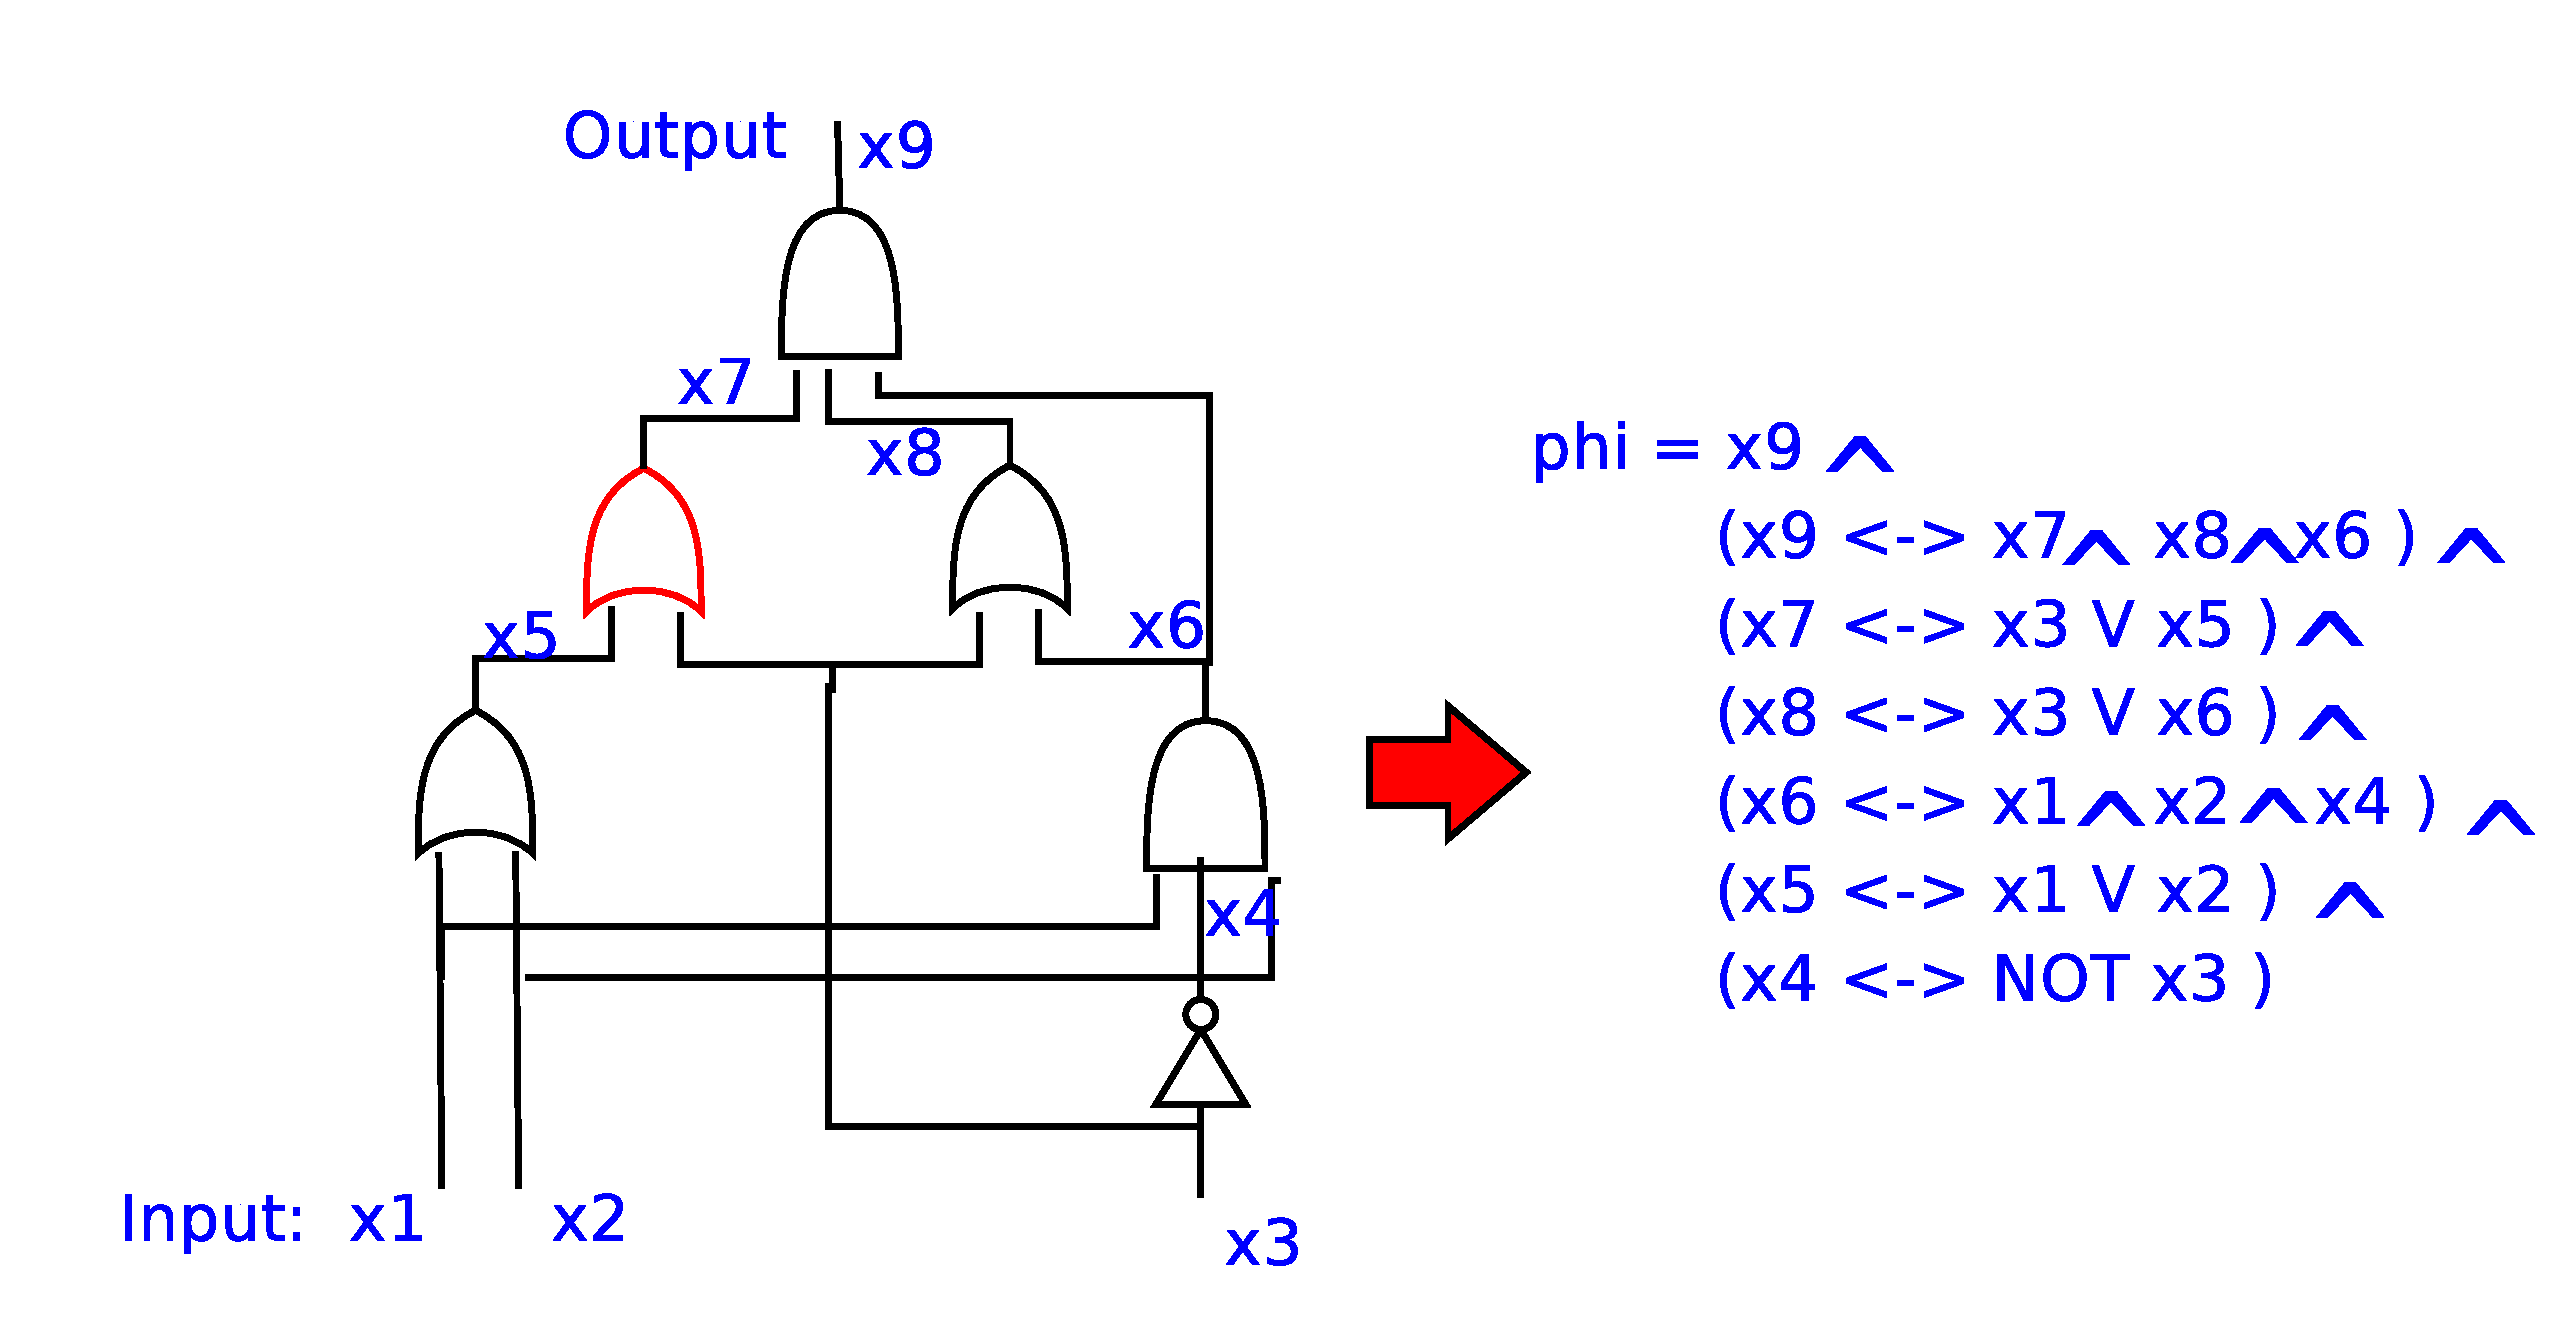
\includegraphics[width=4in]{L4-circuit-to-sat.eps}
\end{figure}
}

\frame{
\begin{Theorem}
 {\sc 3SAT} is NP-Complete. 
\end{Theorem} \footnote{ {\sc 2SAT} belongs to {\bf P}. See slides by D.
Moshko. }
({\sc 3SAT}: each clause has exactly 3 literals.)
\begin{Proof}
\begin{itemize}
 \item 1 literal: $( x_1)$  $ \iff$ $(x_1 \vee p \vee q ) \wedge (x_1 \vee p
\vee \neg q ) \wedge (x_1 \vee \neg p \vee q ) \wedge  (x_1 \vee \neg p \vee
\neg q )  $ 
 \item 2 literals:  $( x_1 \vee x_2)$  $ \iff$ $(x_1 \vee x_2 \vee p) \wedge
(x_1 \vee x_2 \vee \neg p)$
 \item 3 literals: simply copy it.
\item  4 literals: \\
$( x_1 \vee x_2 \vee x_3 \vee x_4) $ \\
$\iff$ $( x_1 \vee x_2 \vee p) \wedge ( p \leftrightarrow x_3 \vee x_4) $ \\
$\iff$ $( x_1 \vee x_2 \vee p) \wedge ( \neg p \vee x_3 \vee x_4) \wedge ( p
\vee \neg x_3 ) \wedge ( p \vee \neg x_4)$ ... 
\item and so on....
\end{itemize}
\end{Proof}
}

\frame{
\frametitle{Thus the following problems are NP-Complete.}
\begin{figure}
 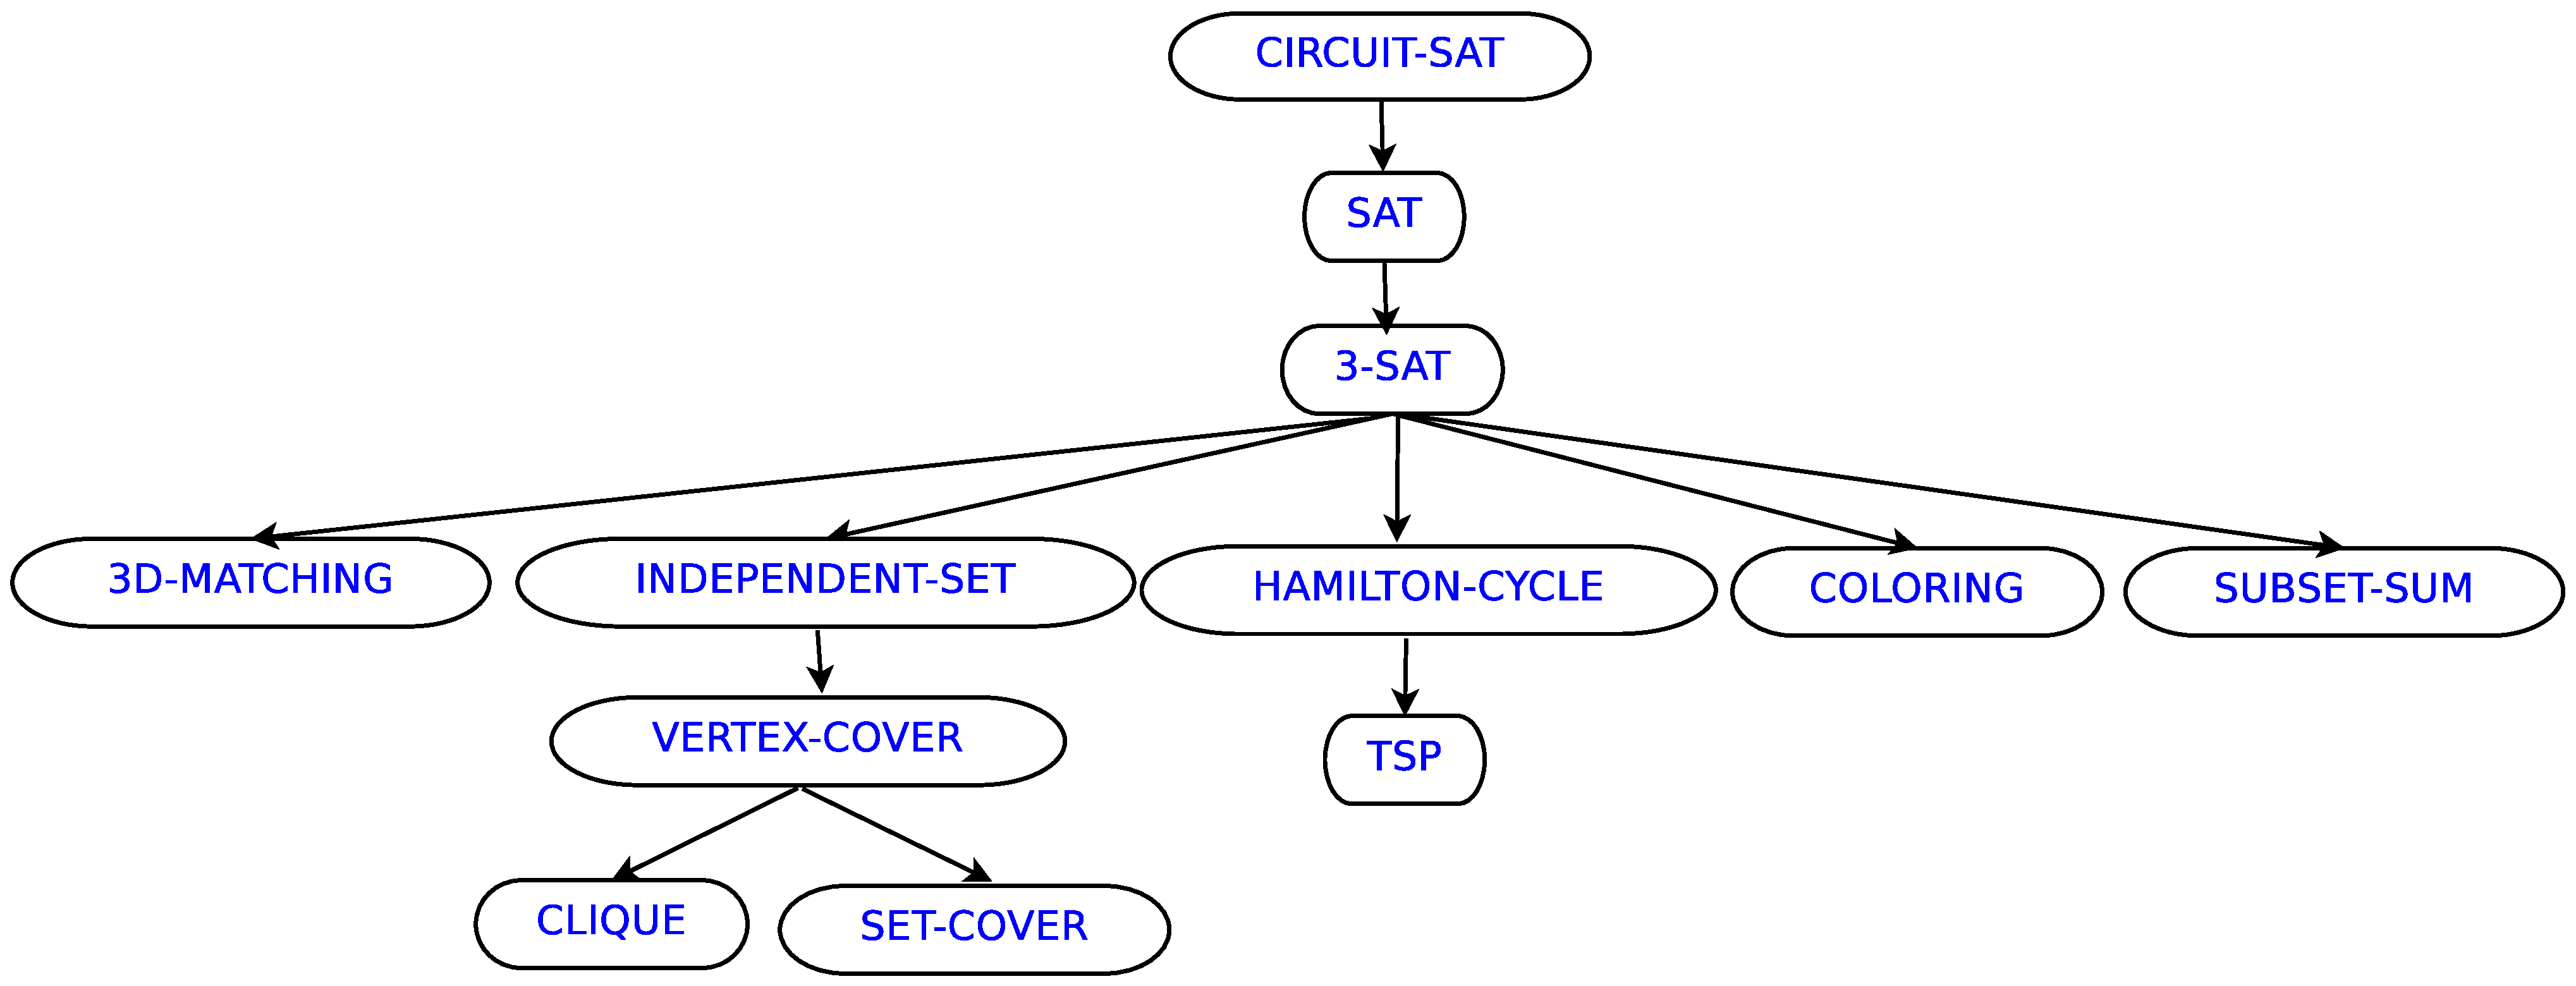
\includegraphics[width=4.5in]{L4-NPC-Tree.eps}
\end{figure}
}


\frame{
\frametitle{A partial taxonomy of hard problems}
 Given a collection of objects,  
\begin{enumerate} 
 \item {\sc Packing} problems: to choose \textcolor{red}{at least} $k$ of them.
Restrictions: conflicts among objects, e.g. {\sc Independent Set}
 \item  {\sc Covering} problems:  to choose \textcolor{red}{at most} $k$ of them to
meet a certain goal, e.g., {\sc Set Cover}, {\sc Vertex Cover}.
 \item  {\sc Partitioning} problems: to divide them into subsets so that each object
appears in exactly one of the subsets, e.g., {\sc 3-Coloring}.  
 \item  {\sc Sequencing} problems: to search over all possible permutations of objects
under restrictions that some objects cannot follow certain others, e.g., {\sc
Hamilton Cycle}, {\sc TSP};
 \item  {\sc Numerical} problems: objects are weighted, to select objects to meet the
constraint on the total weights, e.g., {\sc Subset Sum}
 \item  {\sc Constraint satisfaction} problems. e.g., {\sc 3SAT}, {\sc Circuit
Satisfiability}.
\end{enumerate} 
}


\frame{
\frametitle{}
\begin{block}{}
 The asymmetry of {\bf NP} and {\bf coNP}
\end{block}
}

\frame{
\frametitle{The asymmetry of {\bf NP}}
{\bf NP} is fundamentally asymmetry since: 
\begin{itemize}
 \item For a ``Yes'' instance, we can provide a short ``certificate'' to support
it is ``Yes'';
 \item But for a ``No'' instance, no correspondingly short ``Disqualification''
is guaranteed; 
\end{itemize}
Example: $SAT$ vs. $UNSAT$. \\
\begin{itemize}
\item Certificate of a ``Yes'' instance: an assignment; \\
\item  Disqualification of a ``No'' instance: ? 
\end{itemize}

Example: {\sc Hamilton Cycle} vs. {\sc No Hamilton Cycle} \\
\begin{itemize}
 \item Certificate of a ``Yes'' instance: a permutation of nodes; \\
 \item Disqualification of a ``No'' instance: ?
\end{itemize}
}

\frame{
\frametitle{Problem $X$ and its complement $\bar{X}$}

\begin{itemize}
 \item 
$\bar{X}$ has different property: $s$ is a ``Yes'' instance of $ \bar{X}$ iff
for \textcolor{red}{ALL} $t$ of length at most $p(|s|)$, we have $C(s,t)=No$. 
\item 
co-NP: the collection of $X$ if $\bar{X}$ is in {\bf NP}. \\

\end{itemize}
Example: $UNSAT$, {\sc No Hamilton Cycle}. 

\begin{figure}
 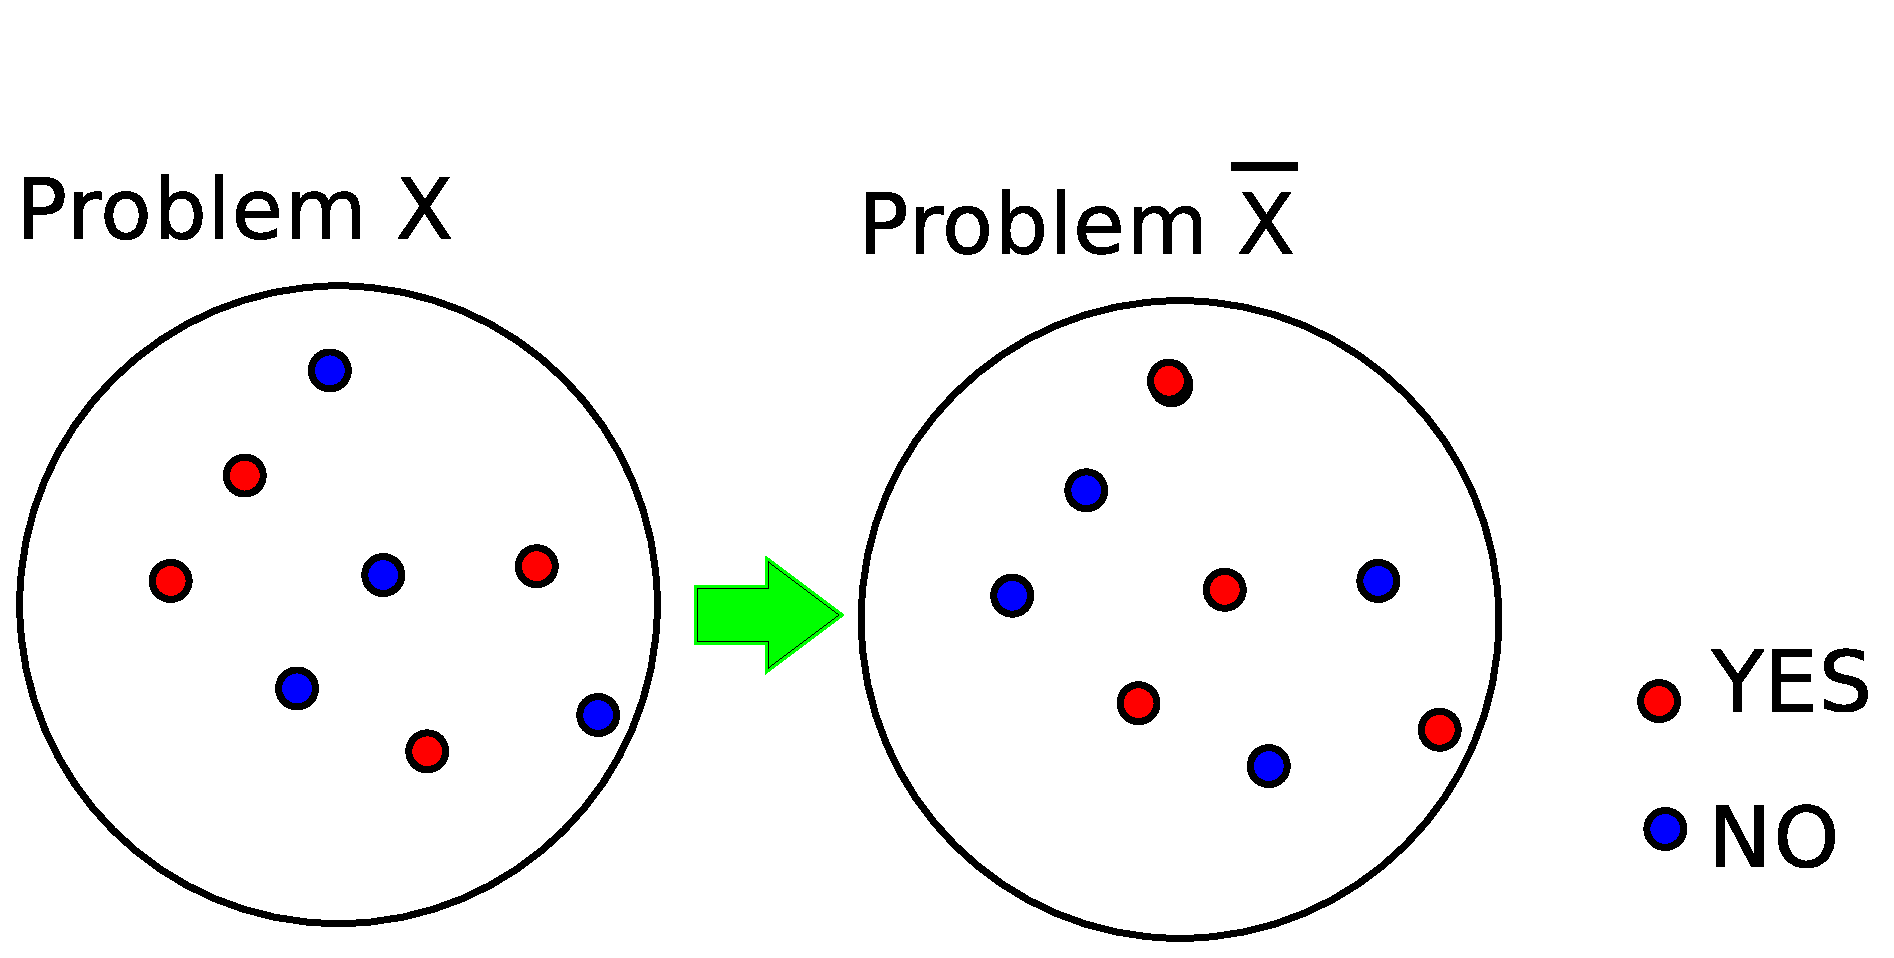
\includegraphics[width=4in]{L3-decisionproblem-X-CoX.eps}
\end{figure}

}

\frame{
\begin{block}{ Question 2: {\bf NP}  = {\bf coNP}? } 
 If yes, then the existence of short certificates for ``Yes'' instances means
that we can find short disqualifications for all ``No'' instances. 
\end{block}
}

\frame{
\frametitle{{\bf NP}  = {\bf coNP}?}
\begin{itemize}
 \item 
Widespread belief: No. 
 \item Just because we have a short certificate for all ``Yes'' instances, it is
not clear why we should believe that the ``No'' instances also have a short
certificate. 
\item 
Proving {\bf NP=coNP} is a bigger step than {\bf P=NP}. 
\end{itemize}
\begin{theorem}
{\bf P=NP} $\Rightarrow$ {\bf NP=coNP}. 
\end{theorem}
\begin{Proof}
\begin{itemize}
 \item 
 Key idea: {\bf P}  is closed under complementation, i.e., $X \in P
\Leftrightarrow \bar{X} \in P$. 
 \item 
$X \in{\bf NP} \Rightarrow X \in P \Rightarrow \bar{X} \in P \Rightarrow 
\bar{X} \in{\bf NP} \Rightarrow X \in  {\bf coNP} $, and 
\item 
$X \in co-NP \Rightarrow \bar{X} \in{\bf NP} \Rightarrow \bar{X} \in P
\Rightarrow X \in P \Rightarrow X \in NP$. 

\end{itemize}
\end{Proof}
}

\frame{
\frametitle{Good characterizations: the class $ {\bf NP} \cap  {\bf coNP} $ }

If $X$ is in both {\bf NP}  and {\bf coNP}, it has a nice property:
\begin{enumerate}
 \item 
 if an instance is ``Yes'' instance, we have a short proof; 
\item 
if the input instance is a ``No'' instance, we have a short disqualification,
too. 
\end{enumerate}
Example: {\sc Maximum Flow}
\begin{itemize}
 \item 
Certificate for ``Yes'' instance: list a flow of value $\ge v$ directly; 
 \item 
Certificate for ``No'' instance: list a cut whose capacity $\le v$; 
\end{itemize}
Duality immediately implies that both problems are in {\bf NP}  and $coNP$. 
} 


\frame{ 
\begin{block}{Question 3: ${\bf P} ={\bf NP} \cap  {\bf coNP} $? }
 If yes, a problem with good characterization always has an efficient algorithm.
\end{block}

} 


\frame{ 
\frametitle{Good characterizations: the class $ {\bf NP} \cap  {\bf coNP} $ }


Mixed opinions: 
\begin{itemize}
\item finding good characterization is usually easier than designing an
efficient algorithm;
\item good characterization $\Rightarrow$ conceptual leverage in reasoning about
problems;
\item good characterization $\Rightarrow$ efficient algorithm: There are many
cases in which a problem was found to have a nontrivial good characterization;
and then (sometimes many years later) it was discovered to have a
polynomial-time algorithm. 
\end{itemize}

Examples: \\
--- linear programming [Khachiyan 1979] \\
--- primality testing [Agrawal-Kayal-Saxena, 2002] 

\footnote{These slides are excerpted from the presentation by Kevin Wayne.}
}

\frame{
\frametitle{Four possibilities for the relationships among {\bf P}, {\bf NP},
and {\bf coNP}.}
\begin{figure}
 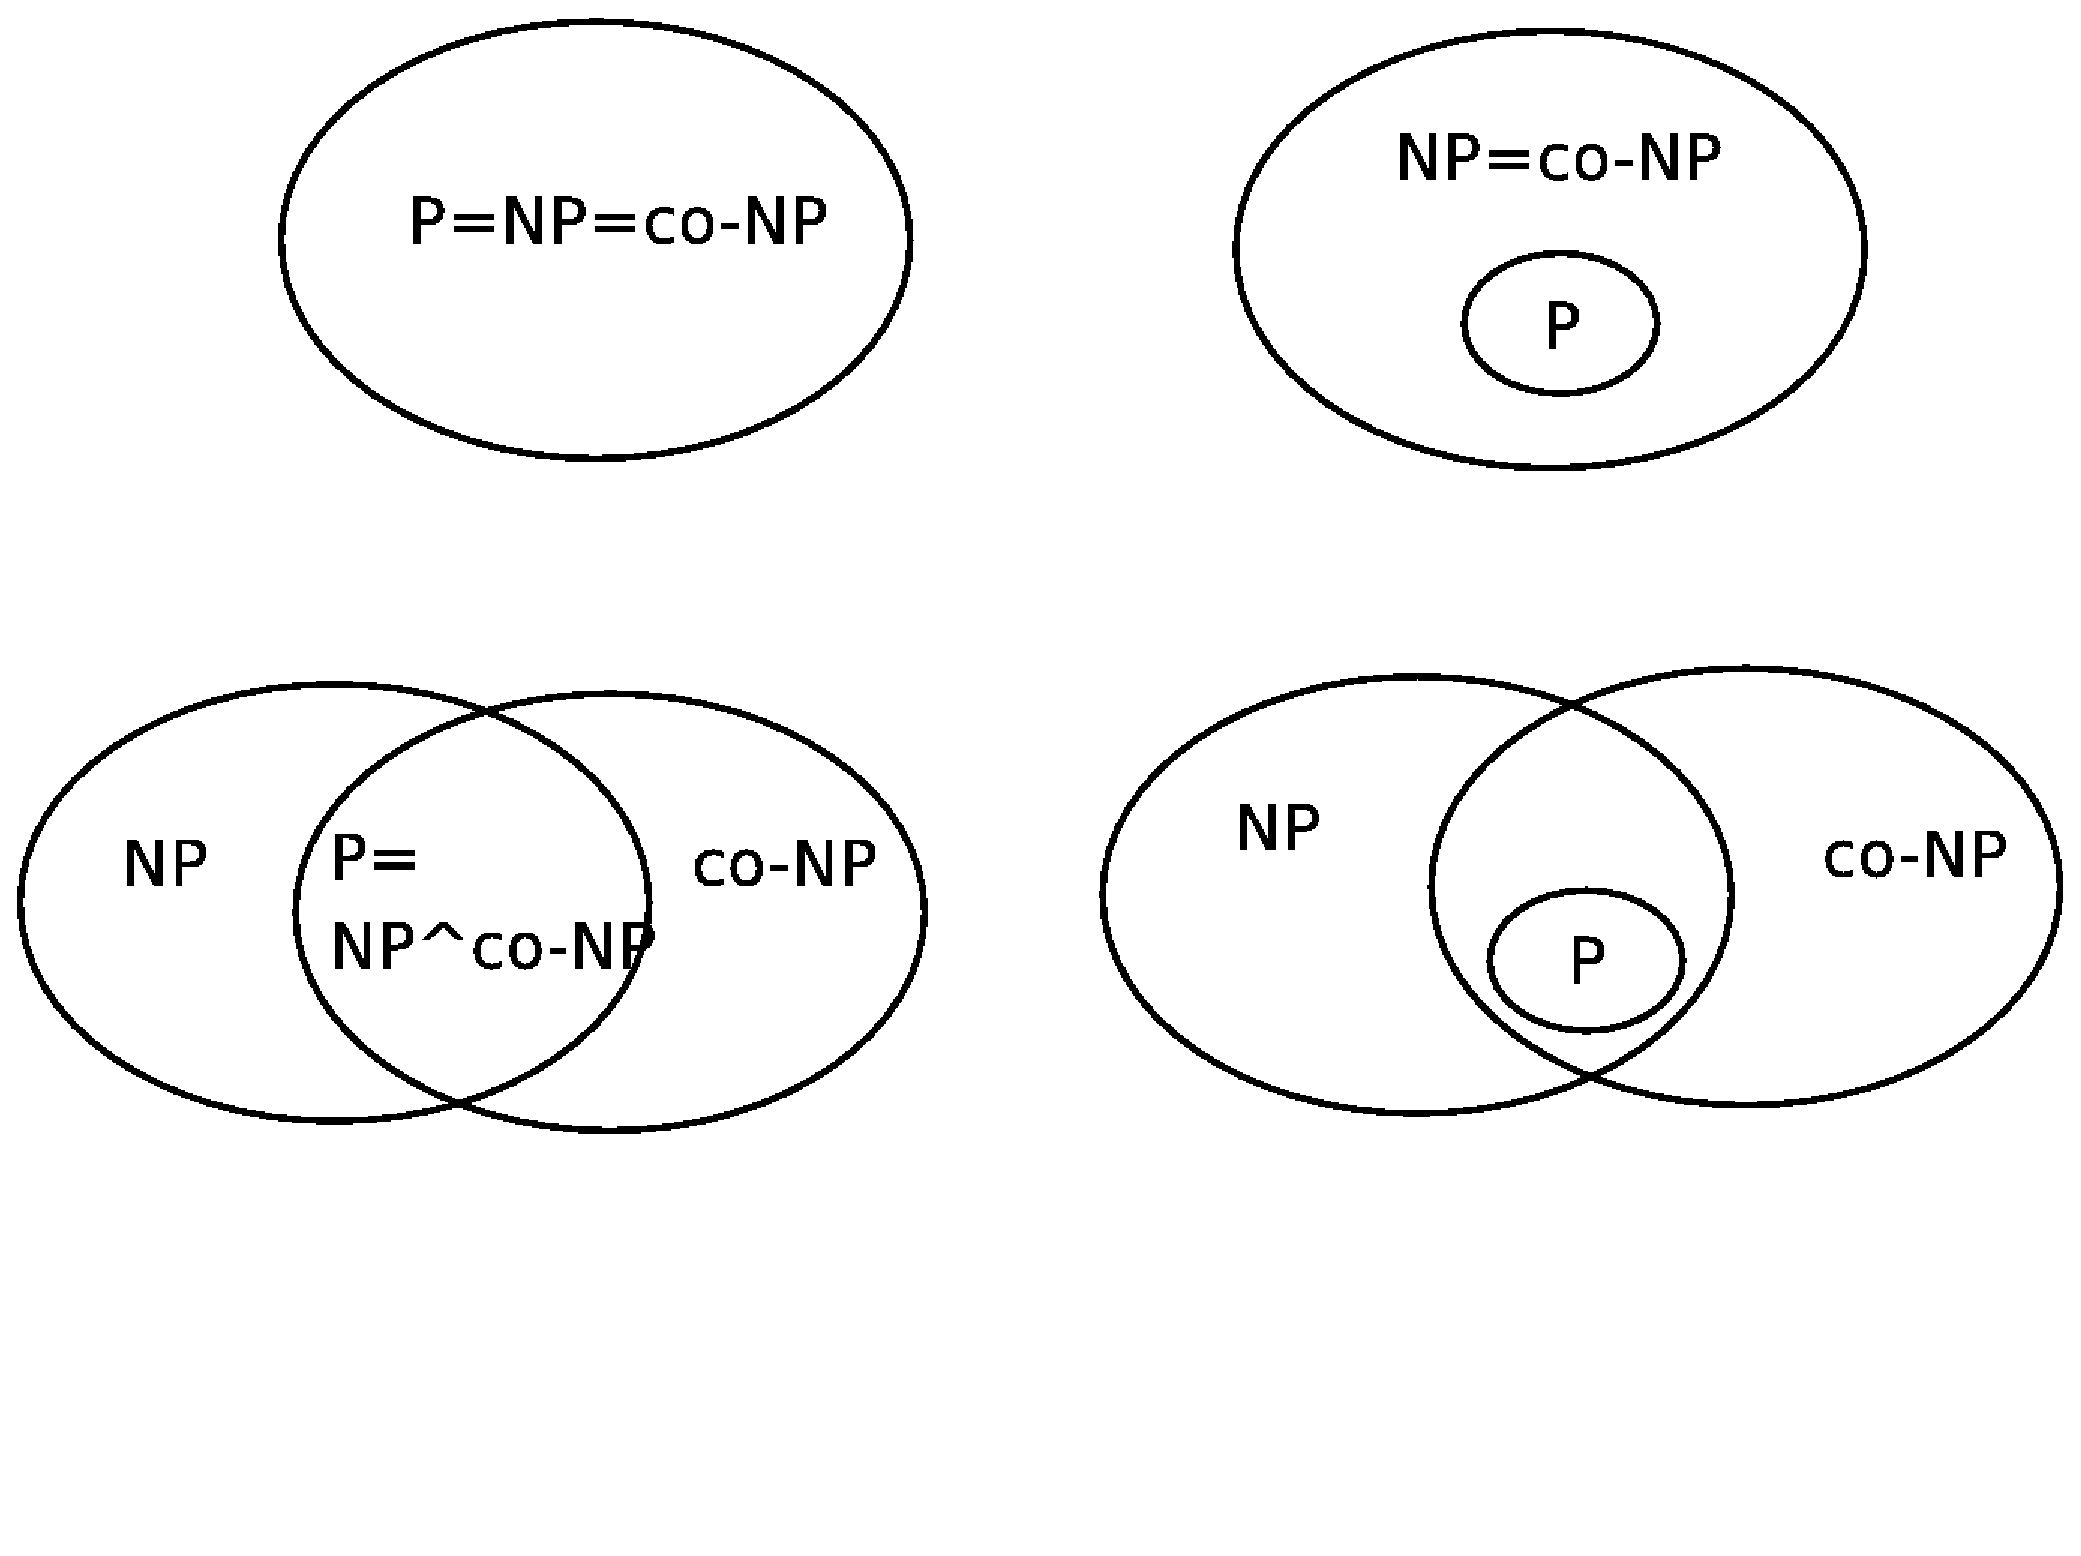
\includegraphics[width=3in]{L4-PNPco-NP.eps}
\end{figure}
}
%
%\frame{
%\begin{block}{Two problems: description and {\bf NP-complete}ness proof}
% \begin{enumerate}
%  \item {\sc Storage Compression} problem: contributed by Xingkui Liu (Data
%Center group, ICT), one proof by Dongbo Bu, and the other proof by Haicang
%Zhang. 
%   \item {\sc Minimum 3D Chip Failure } problem: contributed by Yuanqing Cheng
%(CPU Design  group, ICT), a proof by Haicang Zhang. 
%
% \end{enumerate}
%
%\end{block}
%
%}

\end{document}
